\documentclass[a4paper,12pt]{article}
\usepackage[dvipsnames]{xcolor}
\usepackage{etoolbox} \usepackage[english]{babel} \usepackage[utf8]{inputenc} \usepackage{amsmath} \usepackage{amsfonts} \usepackage{amsthm} \usepackage{graphicx} \usepackage[colorinlistoftodos]{todonotes} \usepackage{amsfonts} \usepackage{bbm} 
\usepackage{setspace} 
\usepackage{enumitem}
\usepackage{pdfsync} \usepackage{xr}
\usepackage[ruled]{algorithm2e}
\usepackage{tikz}
\usepackage{caption}
\usepackage{subcaption}
\usepackage[margin=0.9in]{geometry}
% \usepackage{authblk} % NEW!!!
% \bibliographystyle{econometrica}

\bibliographystyle{plainnat}
\usepackage{hyperref}       % hyperlinks
\hypersetup{
    colorlinks=True,
    citecolor=blue,
    linkcolor=blue,
    filecolor=blue,      
    urlcolor=blue,
    pdftitle={RFP},
    pdfpagemode=FullScreen,
    }

\usepackage{natbib}

\newtheorem{theorem}{Theorem}[section] \newtheorem{proposition}{Proposition}[section] \newtheorem{lemma}{Lemma}[section]

% \newtheorem{definition}{Definition}[section]
\newtheorem{example}{Example} \newtheorem{corollary}{Corollary}[section] \newtheorem{remark}{Remark}[section] \newtheorem{assumption}{Assumption} \newcommand{\citeposs}[1]{\citeauthor{#1}'s \citeyearpar{#1}} \newcommand\fnote[1]{\captionsetup{font=small}\caption*{#1}}

%\usepackage[a4paper,left=3cm,width=14cm,right=3cm]{geometry}
%\def\qed{\rule{2mm}{2mm}} \parskip = 1.5ex
%\textwidth 7in
%\textheight 10 in
%\oddsidemargin -0.4 in
%\evensidemargin -0.4in
%\topmargin -0.7in
\setlength{\parindent}{2em}
\setlength{\parskip}{0.5em}
\renewcommand{\baselinestretch}{1.15}




\begin{document}


\begin{titlepage}
\title{A Deep Learning Assessment of the Right to Counsel}
%\shortTitle{Short title for running head}

\author{Patrick Power, Shomik Ghosh and Markus Schwedeler \\ 
\textcolor{red}{DRAFT}}
\date{\today}
\maketitle
\thispagestyle{empty} % makes the title page number not appear
\vspace{-2em}
\begin{abstract}
Drawing from the Deep Learning Literature and in the language of Category Theory, we introduce a simple and unified structure that generalizes ordinary least squares, allows for nonparametric cluster effects,\footnote{To elaborate on this point, indivduals in the data are grouped together in some fashion. In our context, this grouping is done via a shared zip code. We indicate this grouping via an indicator variable. The nonparametric component is that we allow these the effect of this group memebership on the outcome of interest to vary across the other controls/features. That is, we don't place a functional form assumption on the way the cluster indicator variable interacts with the other controls.} and is inherently compositional, even under regularization. With this framework, we examine the effects of the Right to Counsel: a policy which ensures that low-income households facing eviction have access to free legal representation. Complimenting the existing Economic Literature on the topic, we consider the extent to which the policy makes it harder for low-income individuals to find housing. As some have suggested, if the Right to Counsel increases the cost of evicting a tenant, landlords might respond by making it more difficult to rent a unit in the first place. Exploiting the staggered roll-out of the policy across the state of Connecticut, our preliminary results suggest that on average, housing is harder to secure. 
\vspace{0.2in}\\
\noindent\textbf{Keywords:} Right to Counsel, Evictions, Deep Learning\\
%\noindent\textbf{JEL Codes:} key1, key2, key3\\
\end{abstract}
\setcounter{page}{1}
\end{titlepage}

%\thispagestyle{empty}

%\pagebreak \newpage


%\oneandhalfspacing
\subsection*{The Policy}
In this paper, the term \textit{The Right to Counsel} refers to a policy initiative which ensures that tenants have access to free legal representation in eviction cases. Unlike criminal cases in the U.S., defendants in an eviction case are not provided with a public attorney. Currently, a gap in legal representation exists between landlords and tenants which \cite{collinson2022eviction} has documented to be as large as $95\%-1\%$ in some areas in favor of the landlord.

\section{Introduction}
The 2 million evictions that occur each year across the United States are costly to individuals, landlords, courts, and the general public. Given the severity of these costs, the multitude of factors which contribute to an eviction filling, and the typical manner in which eviction cases are settled, many in the U.S. believe that free legal counsel should be provided to households facing eviction. And indeed, over the past five years, $15$ cities and $3$ states have acted on this belief, initiating a Right to Counsel in some form for low-income households, with additional localities starting pilot studies in the hope of closing the gap in legal representation and improving outcomes. \par 
To some extent, this hope has been empirically justified when considering the direct outcomes of eviction cases. Both in the context of small scale randomized control trials as well as in city-wide roll-outs, researchers have generally found positive results with \cite{seron2001impact}  writing that ``Represented tenants are much less likely to have a final judgment and order of eviction against them'' and \cite{cassidy2022effects} reporting that ``Tenants with lawyers are considerably less likely to be subject to possessory judgments.''\footnote{\cite{greiner2012limits} examines the outcomes of two small scale, Massachusetts based, randomized control trials and finds a measurable impact of legal representation in only one of the trials.} \par 
The concern, though, is that the indirect effects of the policy might diminish or possibly outweigh these positive legal outcomes. Specifically, the concern is that landlords might respond to the policy by making it harder for low-income households to find housing in the first place. As \cite{gunn1995eviction} writes, ``By increasing landlords' costs of doing business, legal services attorneys may enrich their clients at the expense of all other similarly situated poor tenants." And indeed the increase in costs is one of the most consistent findings across the literature as legal services have been shown to increase the duration of eviction proceedings.\footnote{For example, in reference to the duration of eviction proceedings in New York City,  \cite{cassidy2022effects} writes that: ``The number of days between a case filing and a judgment is also significantly longer in the UA zip codes after program implementation.''} The open policy question, then, is the extent to which landlords pass on these perceived costs, and whether these costs are shifted to those who are least able to bear them.\footnote{A lawyer who specializes in evictions wrote via email that `The thing to remember is that higher costs for landlords always get passed on to the tenants in some form (higher rent, deposits, fees, etc.), or the property gets sold, thereby reducing inventory and resulting in higher rents.''} Up to this point, there has been little to no empirical work on this question. \par 
There are two distinct reasons for why up to this point, the above remains an open question. The first is that as \cite{abramson2021welfare} writes, there hasn't been a suitable context to empirically assess the effects at scale. Many of the city wide-roll of the policy overlapped with the eviction moratorium. Only within the past year, as Washington and Connecticut have adopted the policy at the state level has the possibility of estimating the effects at scale become feasible.The second reason is that the adverse effects of the Right to Counsel are likely difficult to measure. Given the informal nature of evictions, -- Mathew Desmond suggests in his New York Times Best Seller, \textit{Evicted}(\cite{desmond2016evicted}), that informal evictions account for $48\%$ of forced moves while formal evictions account for $24\%$ -- landlord's response to the policy may be hard to detect using conventional data sets. For example, landlords might respond by asking for a higher security deposits, requiring additional months of rent upfront or increasing screening standards. \par 
This paper takes a ``noisy'' first step towards addressing both of these issues. First, it exploits the ongoing rollout of the policy across the state of Connecticut where, due to supply constraints of legal services, only low-income individuals in certain zip codes currently receive free legal aid. Second it makes use of data from the U.S. Department of Housing and Urban Development which measures both the characteristics of individuals experiencing homelessness (race, gender, family structure) as well as their length of their housing search. Importantly, this data set is restricted to households who don't face significant barriers to housing. That is, households who are thought to require only limited and partial support. The search length of these households is arguably a key outcome variable for policy makers. \par 
\subsection{Econometric Framework}
A central challenge with the data in this context, as in the case of many policy evaluation papers, is that treatment is assigned at a level above the unit of interest. Specifically, treatment is assinged at the zip code level, while observations are at the individual level. To account for this issue in a nonparametric mannor, this paper builds off the deep learning papers of (\cite{finn2017model} and \cite{kelly2020learning}) by introducing a conceptually simple way to adjust one's estimator for the presence of clustered data as well as to flexibly control the hypothesis space of the model. The model is further explained in section \ref{sec:framework}, but the essential ideas can be understood with a minimal amount of detail. 

Deep Supervised Learning models, the models fit in this paper, are a subset of machine learning models, that can be consuctrued via the composition of parameterized maps and trainined via gradient descent. 
like most deep learning based models, the estimator can be thought of as the composition of parameterized maps where the parameters are updated using some gradient descent like procedure. What is perhaps a bit distinct is that We start by introducing the model in the language of Category Theory. We do so for three distinct reasons. First, presenting a model in terms of the essentials of category theory (objects, arrows, compositions), provides one with a simple way to understand the model.\footnote{To elaborate further, the model training part is done in the Kleisi Category while inference occurs in the Category of Sets}\footnote{Indeed this language is helpful not only for understanding the model, but how it can be seemlessly evaluated and trained with little effort as highlighted in \cite{frostig2018compiling}} As illustrated below, the model can be thought of, as the composition of partially evaluated functions, even under regularization. For the case of regularization we simple tweak our our definition of composition. Second, the act of composition illustrates that our correction for the presence of clustered data can be thought of as a gradient correct. Third, following \cite{domingos2020every}, this gradient correction interpretation allows us to understand our correction from a kernel methods perspective. Note for visual clarify we assume that composition of functions is of higher precedence than function application.
\begin{align*} 
& \textrm{linearModel} \ \textcolor{blue}{\text{data}} \\
& \textrm{linearModel} \circ \ \textrm{identityMap} \ \textcolor{blue}{\text{data}} \\ 
& \textrm{linearModel} \circ  \big(\textrm{featureMap} \ \textcolor{blue}{\text{data}}\big) \ \textcolor{purple}{\text{params}} \\ 
& \textrm{linearModel} \circ  \big(\textrm{featureMap} \ \textcolor{blue}{\text{data}}\big) \circ \textrm{identityMap} \  \textcolor{purple}{\text{params}} \\ 
& \textrm{linearModel} \circ  \big(\textrm{featureMap} \ \textcolor{blue}{\text{data}}\big) \circ \big(\textrm{clusterMap} \ \textcolor{blue}{\text{data}}\big)  \textcolor{purple}{\text{params}} \\ 
& \textrm{linearModel} >=>  \big(\textrm{featureMap} \ \textcolor{blue}{\text{data}}\big) >=> \big(\textrm{clusterMap} \ \textcolor{blue}{\text{data}}\big)  \textcolor{purple}{\text{params}} \\ 
\end{align*}
 
\subsection{Heterogeneity}
Lastly, while no pre-analysis plan accompanies this paper, the only source of heterogeneity explored is the effects of the policy on Black and female tenants. As well documented in the eviction literature, these subgroups share the greatest likelihood and costs of evictions, as \cite{desmond2019unaffordable} writes, ``Low-income women, especially poor black women, are at high risk of eviction'', and \cite{collinson2022eviction} notes that with regards to the costs of evictions, ``We find particularly sharp negative impacts for female and Black tenants,\footnote{\cite{evans2019reducing} writes `} who drive the effects on labor market outcomes, residential mobility, and interactions with homelessness.'' It seems likely, therefore, that if landlords respond in an adverse way to The Right to Counsel, it would be be towards this sub-population in particular. Hence, all regression specifications are fit both over the entire sample and this sub-sample of interest. 
\subsection{Literature Review}
\begin{itemize}
    \item Not all areas have experienced a decline in homelessness. The trends in New York City (CoC NY600) and Los Angeles County7 have been particularly different from the rest of the country. In Figure 3, the solid lines report homelessness rates (x 100,000) for Los Angeles County and New York City (right vertical
axis). Note that since 2012, these rates have increased by 57 and 31 percent, respectively
\end{itemize}
While this paper certainly engages with various literatures, from statistical discrimination, to applied deep learning, its central aim is to provide additional insight into the effectiveness of the Right to Counsel. \par 
 In line with the recent Economic works on the topic, it does so by offering a partial assessment of the policy ``at scale''. This approach differs significantly from some of the prior randomized control trial studies where only a limited number of judges were involved as in \cite{greiner2012limits} or where only individuals who were thought to likely benefit from legal representation were provided with laywers from private firms working pro bono as in \cite{seron2001impact}.   

In contrast to the recent Economic literature, though, this paper empirically considers the indirect effects of the policy, thereby complementing \cite{cassidy2022effects} which empirically focuses on the direct effects, and \cite{abramson2021welfare} which considers the indirect effects via a counterfactual exercise.


The recent events of Covid-19 and rising inflation have magnified the importance and fragility of housing for low-income individuals. In response to this, we empirically assess the effectiveness of an initiative, growing in popularity across the U.S., known as the Right to Counsel (RTC). Currently adopted in 15 cities and 3 states, the initiative aims to combat the 3.6 million eviction fillings that occur each year in the U.S. by closing the gap in legal representation between landlord and tenant. Closing such a gap entails providing legal representation for tenants which as the case of Boston in 2019 which saw 39,594 eviction cases filed only  with only $8.7\%$ of tenants represented.\footnote{(\href{https://bostonbar.org/app/uploads/2022/06/rtc-report-for-web-or-email.pdf}{Samuelson et a. [2020]})}

 Complimenting both the small, but growing Economic literature on this topic (\cite{abramson2021welfare}, \cite{cassidy2022effects}) and earlier studies based on small scale randomized control trials (\cite{seron2001impact}), we consider the indirect effects of the Right to Counsel policy. Exploiting the recent staggered roll-out across Connecticut, we consider the extent to which the policy may actually increase housing instability by making it harder for those currently unhoused to find permanent housing. As some have suggested, if the policy increases the cost of evicting a tenant,\footnote{Indeed one of the most consistent findings across the literature is the increase in processing time: \cite{cassidy2022effects} writes: ``The number of days between a case filing and a judgment is also significantly longer in the UA zip codes after program implementation.''} landlords might respond by making it harder for low-income individuals to rent a unit in the first place.\footnote{This idea has been emphasized both in the academic literature as as \cite{gunn1995eviction} writes, ``By increasing landlords' costs of doing business, legal services attorneys may enrich their clients at the expense of all other similarly situated poor tenants."  and in personal conversations with lawyers who specialize in evictions: ``The thing to remember is that higher costs for landlords always get passed on to the tenants in some form (higher rent, deposits, fees, etc.), or the property gets sold, thereby reducing inventory and resulting in higher rents.''}

Using individual level data from the U.S. Department of Housing and Urban Development, and fitting a variety of estimators to the data, from difference-in-means to machine learning based estimators, our preliminary estimates suggest while the policy has no noticeable effects on for the average individuals, it may make it more difficult for African American women to find permanent housing. The estimate, while crude and preliminary, maintains a positive sign above $5$ percentage points both across regression specifications as well as across subsets of zip codes. 
Eviction number from \cite{gromis2022estimating}. (Individual Costs): \cite{collinson2022eviction} writes, ``We find that eviction causes significant disruptions that are reflected in increases in residential mobility, homelessness, and hospital use''. (Court Costs): As \cite{seron2001impact} notes, legal representation actually might decrease housing court costs as the number of appearances and post judgement motions decline. (General Public): As \cite{desmond2019unaffordable} writes, ``Residential instability often brings about other forms of instability—in families, schools, communities— compromising the life chances of adults and children''

(Multitude of Causes):  David Ehrens writes in his \href{https://dartmouth.theweektoday.com/article/opinion-support-right-counsel-renters/58185}{letter} to the editor of \href{https://dartmouth.theweektoday.com/}{Dartmouth Week} of ``evictions related to the pandemic, chronic housing supply shortages, inequities in lending, generational poverty, and other harms''. (Eviction Proceedings): \textcolor{blue}{Missing Reference} writes ``the vast majority resolved by default or settlement, typically the result of hallway negotiation'' (Growing Interest): \cite{engler2010connecting} writes ``a renewed call for a civil right to counsel, or civil Gideon, has gained momentum \dots as well as a surge in membership in the newly-created National Coalition for a Civil Right to Counsel.''

\section{Policy Details}
\subsection{Timeline}
In June of 2021, Governor Lamont of Connecticut signed into law the Right to Counsel (3). As highlighted in the timeline below, this event coincides with the end of the local moratorium on evictions (4) in Connecticut. Six months later, on January 31, 2022, as Covid-19 relief was winding down, the Right to Counsel went into effect. A detailed description of the timeline is provided in the appendix, but key dates of interest, including the start and end of local and national moratoriums, are illustrated below. 
\par 
\begin{figure}[htbp]
\centering
    \centering
    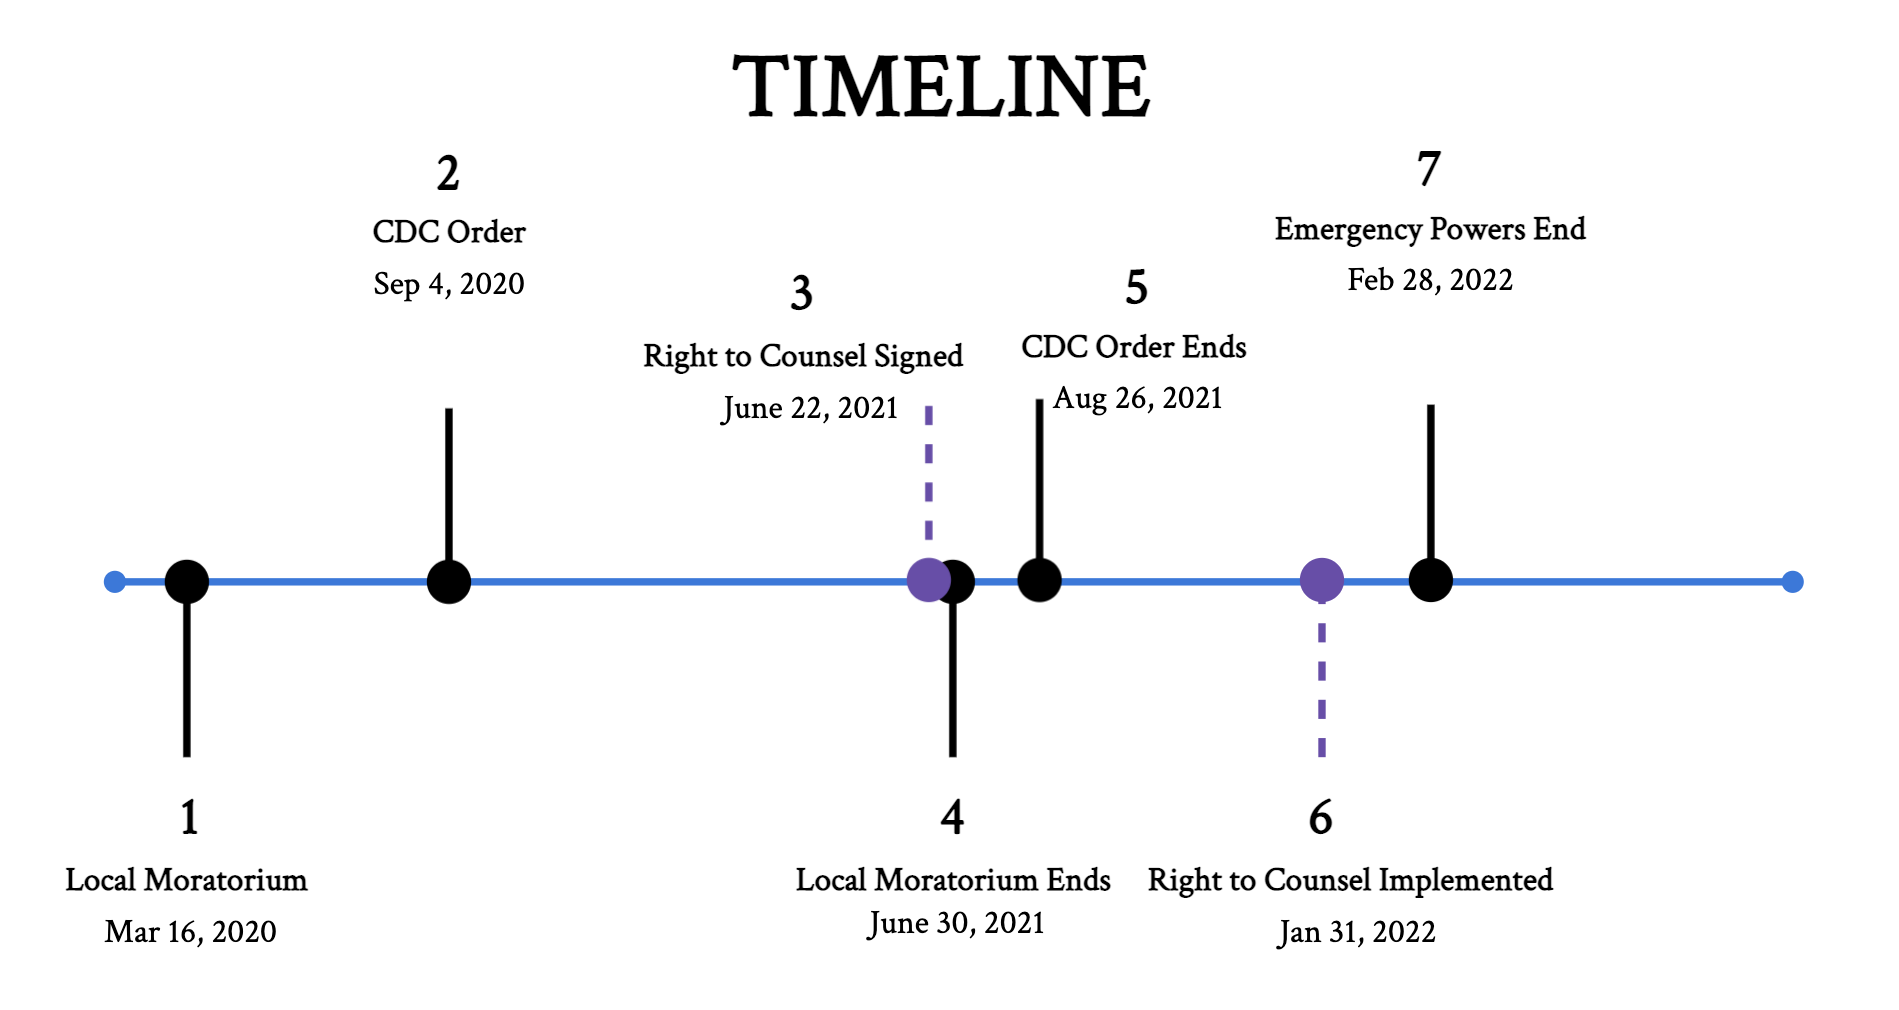
\includegraphics[width=.60\linewidth]{figures/rtc/context/timeline.png}
    %\caption{All zip codes}
    \label{SUBFIGURE LABEL 3}
\end{figure}

\subsection{Implementation}
Because the expected demand for legal services under the Right to Counsel exceed the current level of legal support, state representatives decided to implement the policy in phases.\footnote{During the two years leading up to the pandemic, Connecticut saw 20,000 eviction fillings on average\footnote{\href{https://youtu.be/sLpi4xlVGgU?t=1002}{link}}} In the first stage, the policy was made available to a subset of the zip codes (the 14 shown in yellow) which correspond to $30\%$ of evictions and $20\%$ percent of the renter population.\footnote{CBF Assignment Sheet-- received via email on August 26th --Expected to assist 2,000 households in the first phase, in a state where 20,000 residents faced eviction} Individuals and families within these zip codes who made $80\%$ or less than the area median income were eligible for legal support starting on January 31, 2022.\footnote{(\href{https://www.cga.ct.gov/2021/ACT/PA/PDF/2021PA-00034-R00HB-06531-PA.PDF}{"Income-eligible"} means (A) having household income at or below
eighty per cent of the state median income adjusted for family size, as
determined by the United States Department of Housing and Urban
Development, at the time of the request for representation; or (B)
receiving one of the following types of public assistance: (i) Temporary
Assistance for Needy Families, (ii) Supplemental Nutrition Assistance
Program benefits, (iii) Medicaid, (iv) Supplemental Security Income, (v)
refugee resettlement benefits, (vi) rental assistance under chapter 138a
of the general statutes, or (vii) the federal Housing Choice Voucher
Program, 42 USC 1437f(o); } Beginning earlier, on October 1, 2021, landlords were to notify individuals of the existence of this policy when serving tenants with a notice to quit (the first step in an eviction proceeding -- the entire process is described in more detail in the appendix). In addition to landlords, courts were expected to inform tenants of the policy when and if tenants appeared in court.\footnote{\href{https://www.cga.ct.gov/2021/ACT/PA/PDF/2021PA-00034-R00HB-06531-PA.PDF}{``On} and after October 1, 2021, an owner, lessor, landlord, legal
representative or agent of an owner, lessor or landlord, a housing
authority or a housing subsidy program administrator, as applicable,
shall attach a copy of the notice described under subdivision (1) of this
subsection, to (A) a notice to quit delivered to a covered individual
pursuant to chapter 832 or chapter 412 of the general statutes; (B) a
summons and complaint for a summary process action pursuant to
chapter 832 or chapter 412 of the general statutes; (C) a lease termination
notice for a public or subsidized housing unit; and (D) a notice to
terminate a state or federal housing subsidy''}\footnote{\href{https://www.cga.ct.gov/2021/ACT/PA/PDF/2021PA-00034-R00HB-06531-PA.PDF}{``An}y court notice scheduling a mediation or hearing that is sent to
a self-represented party in a covered matter shall include plain language
information about the availability of legal representation through the
right to counsel program and a phone number for accessing information
and applying for assistance.''} Given that the lack of enforcement with respect to landlords and that $37\%$ of Connecticut tenants fail to appear in court during eviction proceedings, it's quite possible that many eligible tenants are not yet aware of the policy's existence.\footnote{According to \href{https://www.ctpublic.org/news/2022-01-30/some-residents-facing-eviction-could-now-be-eligible-for-free-legal-aid}{article} $37\%$ of Connecticut tenants fail to appear in court during eviction proceedings, and their cases end in default, according to a 2021 report by the Connecticut Advisory Council on Housing Matters.}
\begin{figure}[htbp]
\centering
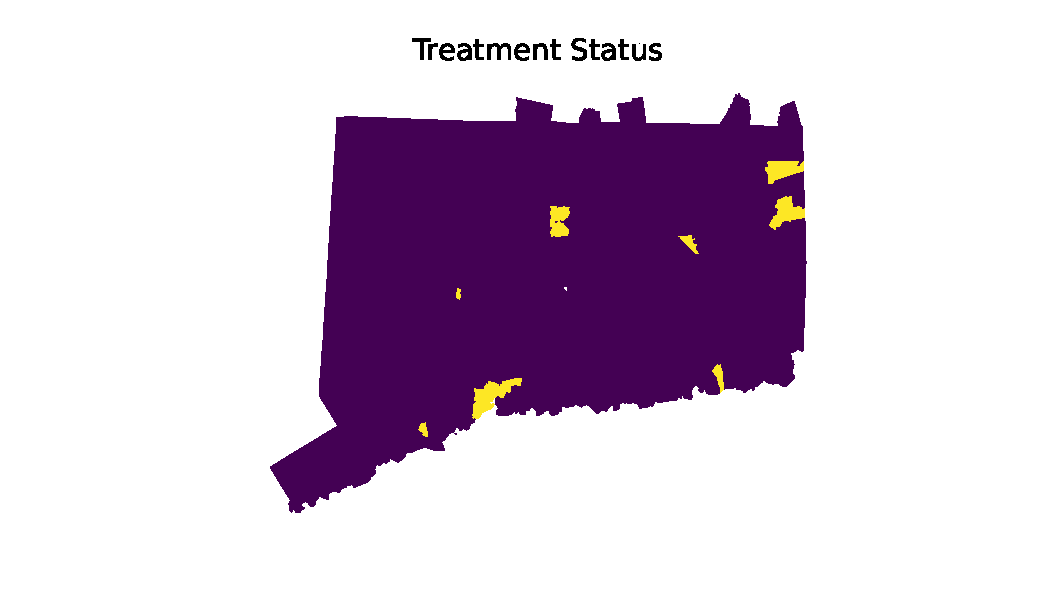
\includegraphics[width=0.7\textwidth]{figures/rtc/maps/zip_code_status.pdf}  
        \caption{Treatment status for each zip code (yellow indicates treated zip code): \href{https://github.com/pharringtonp19/evictions/blob/main/scripts/joint/maps/treatment_status.py}{Reproduced Here}}
\end{figure}

\subsection{Data \& Outcomes}
As referenced prior, the outcome of interest is the search length for households who are currently experiencing homelessness but face limited barriers to housing. Rapid Re-housing, a federally tracked program, provides limited short term assistance to exactly this population.\footnote{As \cite{evans2019reducing} explains, ``The
Homeless Management Information System (HMIS) is a nationwide network of local IT systems that collect
client-level data for people entering sheltered services. These systems are organized at the CoC level and most
homeless shelters across the country are part of the HMIS system''} Its aim is to help ``families exit shelters and get back into permanent housing quickly.''\footnote{\textrm{Missing Source}} While different in nature than an independent housing search, the search length of individuals in a Rapid Rehousing program a reasonable proxy for the following three reasons. First, Rapid Rehousing programs ``serve people experiencing homelessness with no preconditions such as employment, income, absence of criminal record, or sobriety.''\footnote{\href{https://www.urban.org/sites/default/files/publication/99153/rapid_re-housings_role_in_responding_to_homelessness_3.pdf}{Reference}} Second, the program does not target people who might need long-term assistance. Those individuals and families are helped by permanent supportive housing programs.\footnote{Very different from permanent supportive housing which is as Rosanne Haggerty writes in the NyTimes, ``is ideal for those with serious health challenges who have been homeless for long periods of time''.\footnote{\href{https://www.nytimes.com/roomfordebate/2015/02/19/homes-for-the-homeless/for-even-the-neediest-housing-is-the-solution-to-homelessness}{NyTimes}}}\footnote{ \textbf{Cost}: at $\$6,678$ per family, it is cheaper than transitional housing at $\$32,557$ per family.\footnote{\href{https://cceh.org/provider-resources/rapid-rehousing/}{CCEH Video}}} Third, the lease agreement households sign come with ``the same rights and responsibilities as a typical lease holder.''\footnote{\href{thttps://endhomelessness.org/resource/rapid-re-housing-a-history-and-core-components/}{It} is imperative that any lease agreement provides the tenant with **the same rights and responsibilities as a typical lease holder** and that the financial terms of the lease are such that the household has a reasonable ability to assume rental costs once financial support ends (keeping in mind that in the majority of cases, even households with no income at move-in retain their housing)"}
\begin{itemize}
    \item \cite{evans2019reducing}: The Family Options Study provides the primary experimental test of the effectiveness of rapid rehousing (RRH), but the results for this treatment arm are mixed. There were no statistically significant
differences in housing outcomes between the control and short-term subsidy group by the three-year followup. (Gubits et al. 2016).
\end{itemize}
\begin{figure}[htbp]
\centering
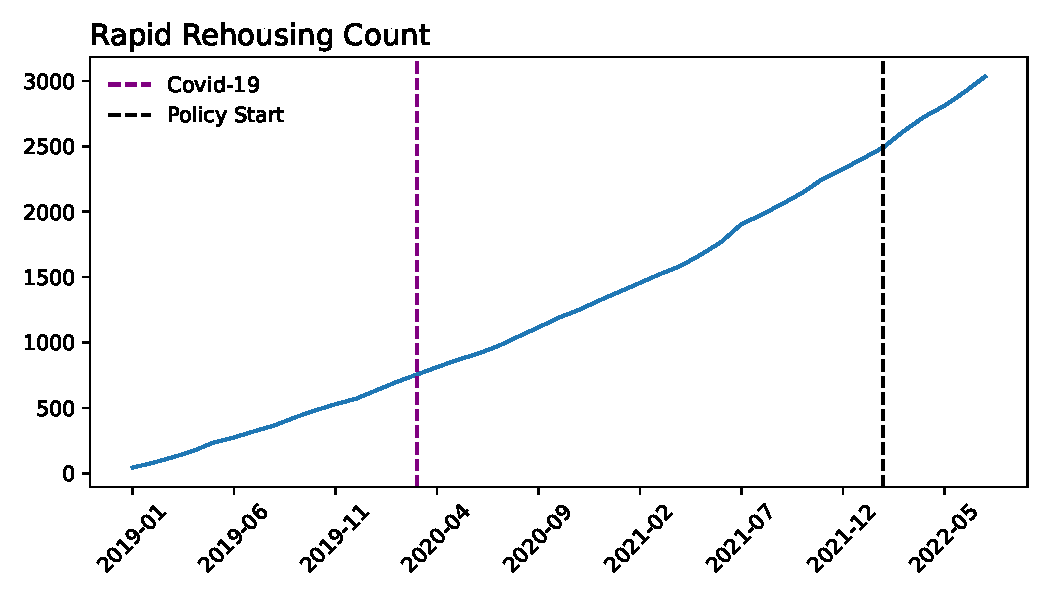
\includegraphics[width=0.7\textwidth]{figures/rtc/context/rrh_counts.pdf}
        \caption{Treatment status for each zip code (yellow indicates treated zip code): \href{https://github.com/pharringtonp19/evictions/blob/main/scripts/cceh/plot/summary_rrh.py}{Reproduced Here}}
\end{figure}
\section{Framework}
\label{sec:framework}
\subsection{Context}
To keep things simple, we describe our approach in the specific context of cluster-level randomized control trials where we're interested in estimating treatment heterogeneity.\footnote{ Cluster-level randomized control trials are randomized control trials where treatment varies at a level above the unit of interest} Such experiments are common in development, education, and health settings because they are (A) generally easier to implement, (B) better adhere to the potential outcome framework\footnote{Reduce the chance of spillover effects between treated and non-treated individuals.} and perhaps most importantly\footnote{See John Lists's book, `The Voltage Effect` which highlights this importance in great detail} (C) allow us to understand the the effects of scaling the treatment.\footnote{Many large scale studies such as HIE prefer to include many control variables in their regression specification: size of family, age categories, education level, income, self-reported health status, and use of medical care in the year prior to the start of the experiment, kind of insurance (if any) the person had prior to the experiment, whether family members grew up in a city, suburb, or town, and spending on medical care and dental care prior to the experiment} With a binary treatment variable, such a problem can be decomposed into two separate problems where the objective function is minimized separately over the treatment and control groups.

\begin{align*}
    \underset{f \in \sigma(X)}{\text{inf}} \ E\big[(Y - f)^2\big]
\end{align*}
 

\subsection{Challenge (\textcolor{blue}{The Tragic Triad})\footnote{The expression "tragic triad" is taken from Gradient Surgery for Multi-Task Learning}}
Under the potential outcome framework, clustered level treatment assignment can be roughly thought of as forming the treatment and controls groups via random clustered sampling. From an estimation standpoint, this poses a few challenges because in each treatment group: We observe only a subset of the clusters; The distribution of covariates can differ across clusters; The distribution of outcomes conditional on covariates may differ across clusters. The above issues are perhaps only magnified as we increase the dimensionality of the data.\par 
As shown in figure \ref{fig:high}, we extended the work of \cite{balestriero2021learning} to the situation of clustered sampling. As illustrated in figure \ref{fig:higha}, clustered sampling doesn't change the fundamental issue of learning in high dimensions: extrapolation. It does, however, as indicated in figure \ref{fig:highb}, suggest that we may need to reconsider how we go about learning in this context
\begin{figure}[htbp]
\centering
\begin{subfigure}{.48\textwidth}
    \centering
    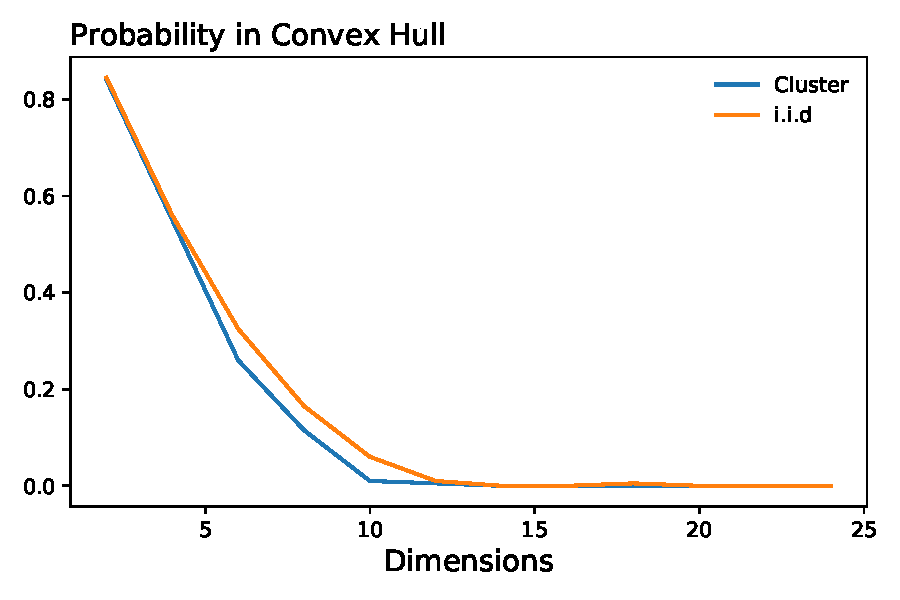
\includegraphics[width=.95\linewidth]{figures/framework/iid_cluster.pdf}
    \caption{}
    \label{fig:higha}
\end{subfigure}
\begin{subfigure}{.48\textwidth}
    \centering
    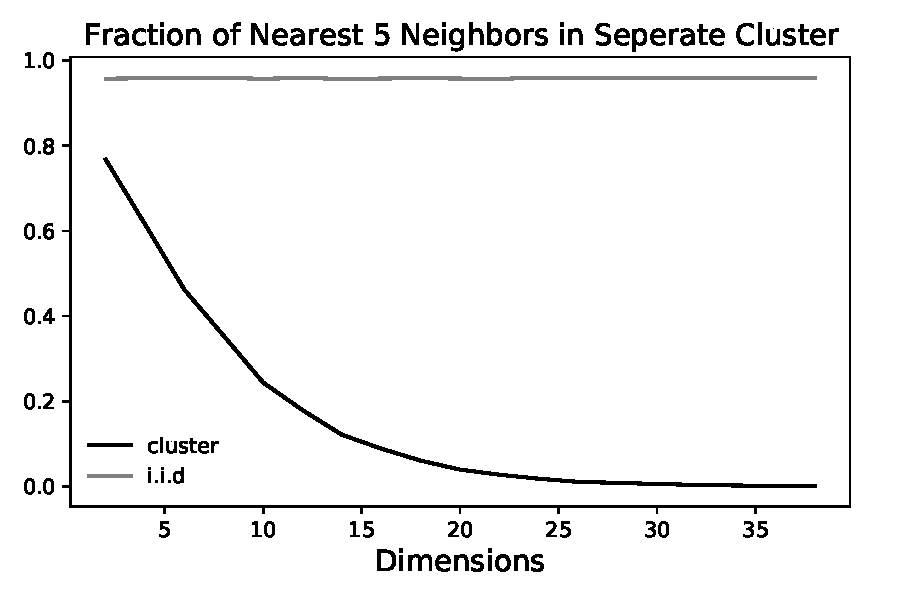
\includegraphics[width=.95\linewidth]{figures/framework/nearest_neighbors_increasing_correlation.pdf}
    \caption{}
    \label{fig:highb}
\end{subfigure}
\caption{}
\label{fig:high}
\end{figure}



The central challenge is how to incorporate a cluster indicator in the training phase so that the function adaptively pools information across clusters, without using the cluster indicator in the inference phase. To highlight this, we construct a toy data set where the average within cluster outcome value is zero (i.e. adding cluster specific fixed effects would not improve the fit to the data). The central challenge is how ``addaptively'' share information across clusters. That is, when there are a lot of clusters present, we would intuitively prefer a small bandwidth. When there are few clusters present, we would prefer a larger bandwidth. And of course, we would like to extend this to high dimensions.

\begin{figure}[htbp]
\centering
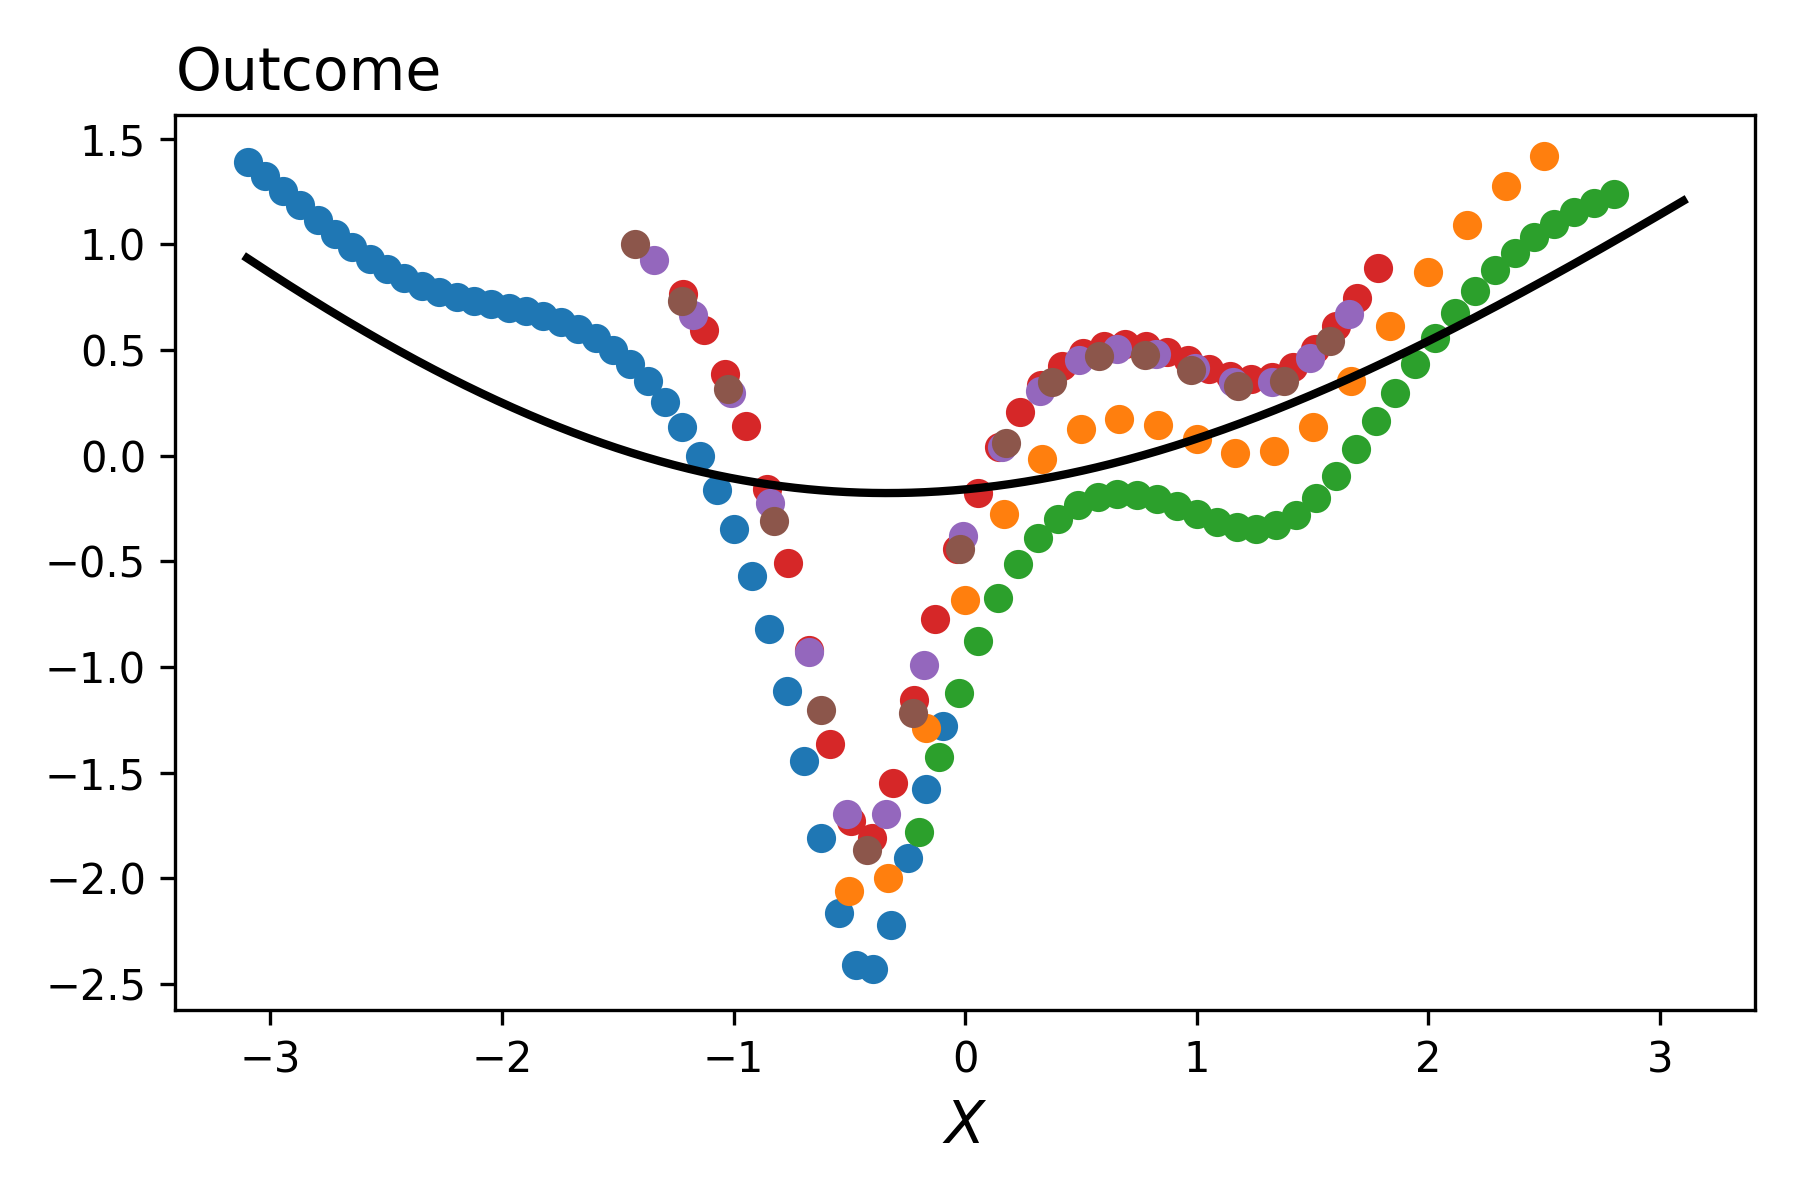
\includegraphics[scale=0.3]{figures/framework/local_linear_no_const_0.5_18_LM.png}
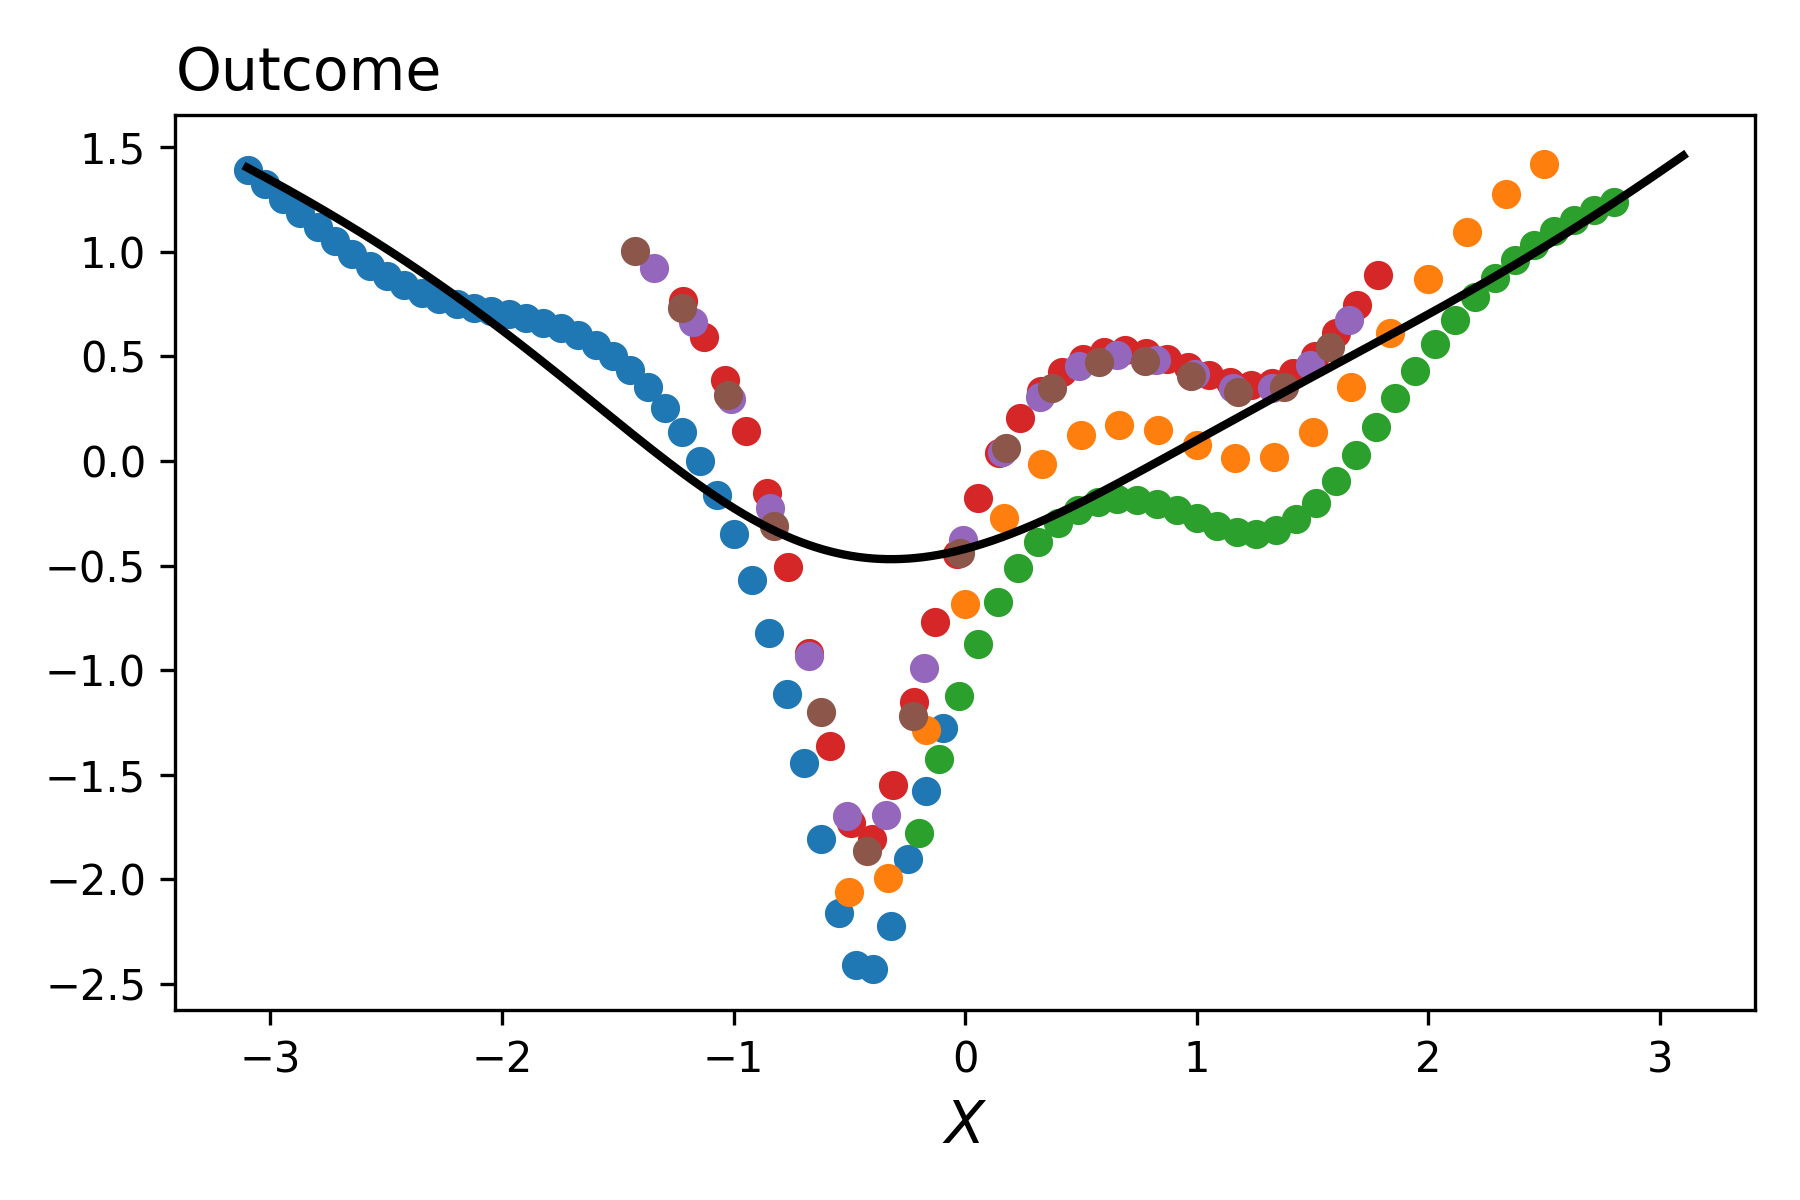
\includegraphics[scale=0.3]{figures/framework/local_linear_no_const_1.0_18_LM.png}
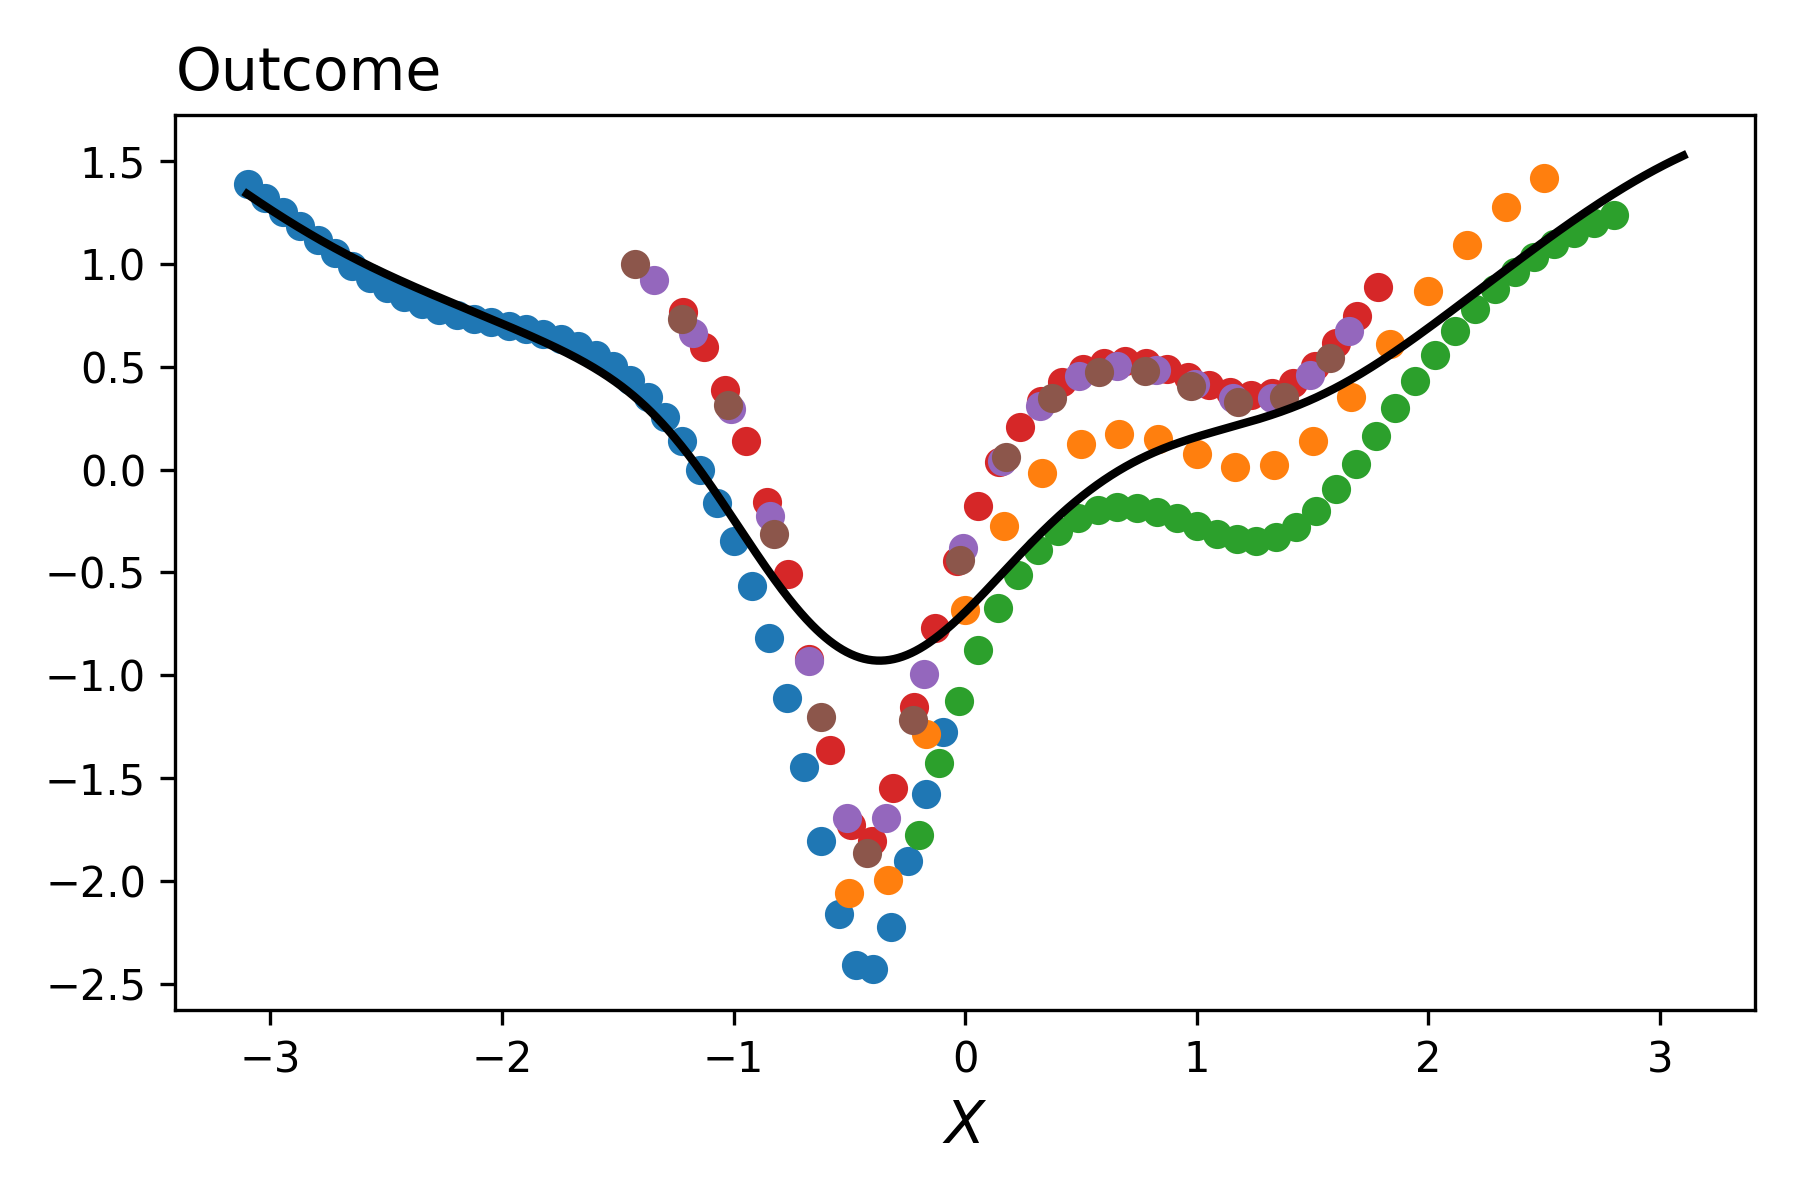
\includegraphics[scale=0.3]{figures/framework/local_linear_no_const_2.0_18_LM.png}
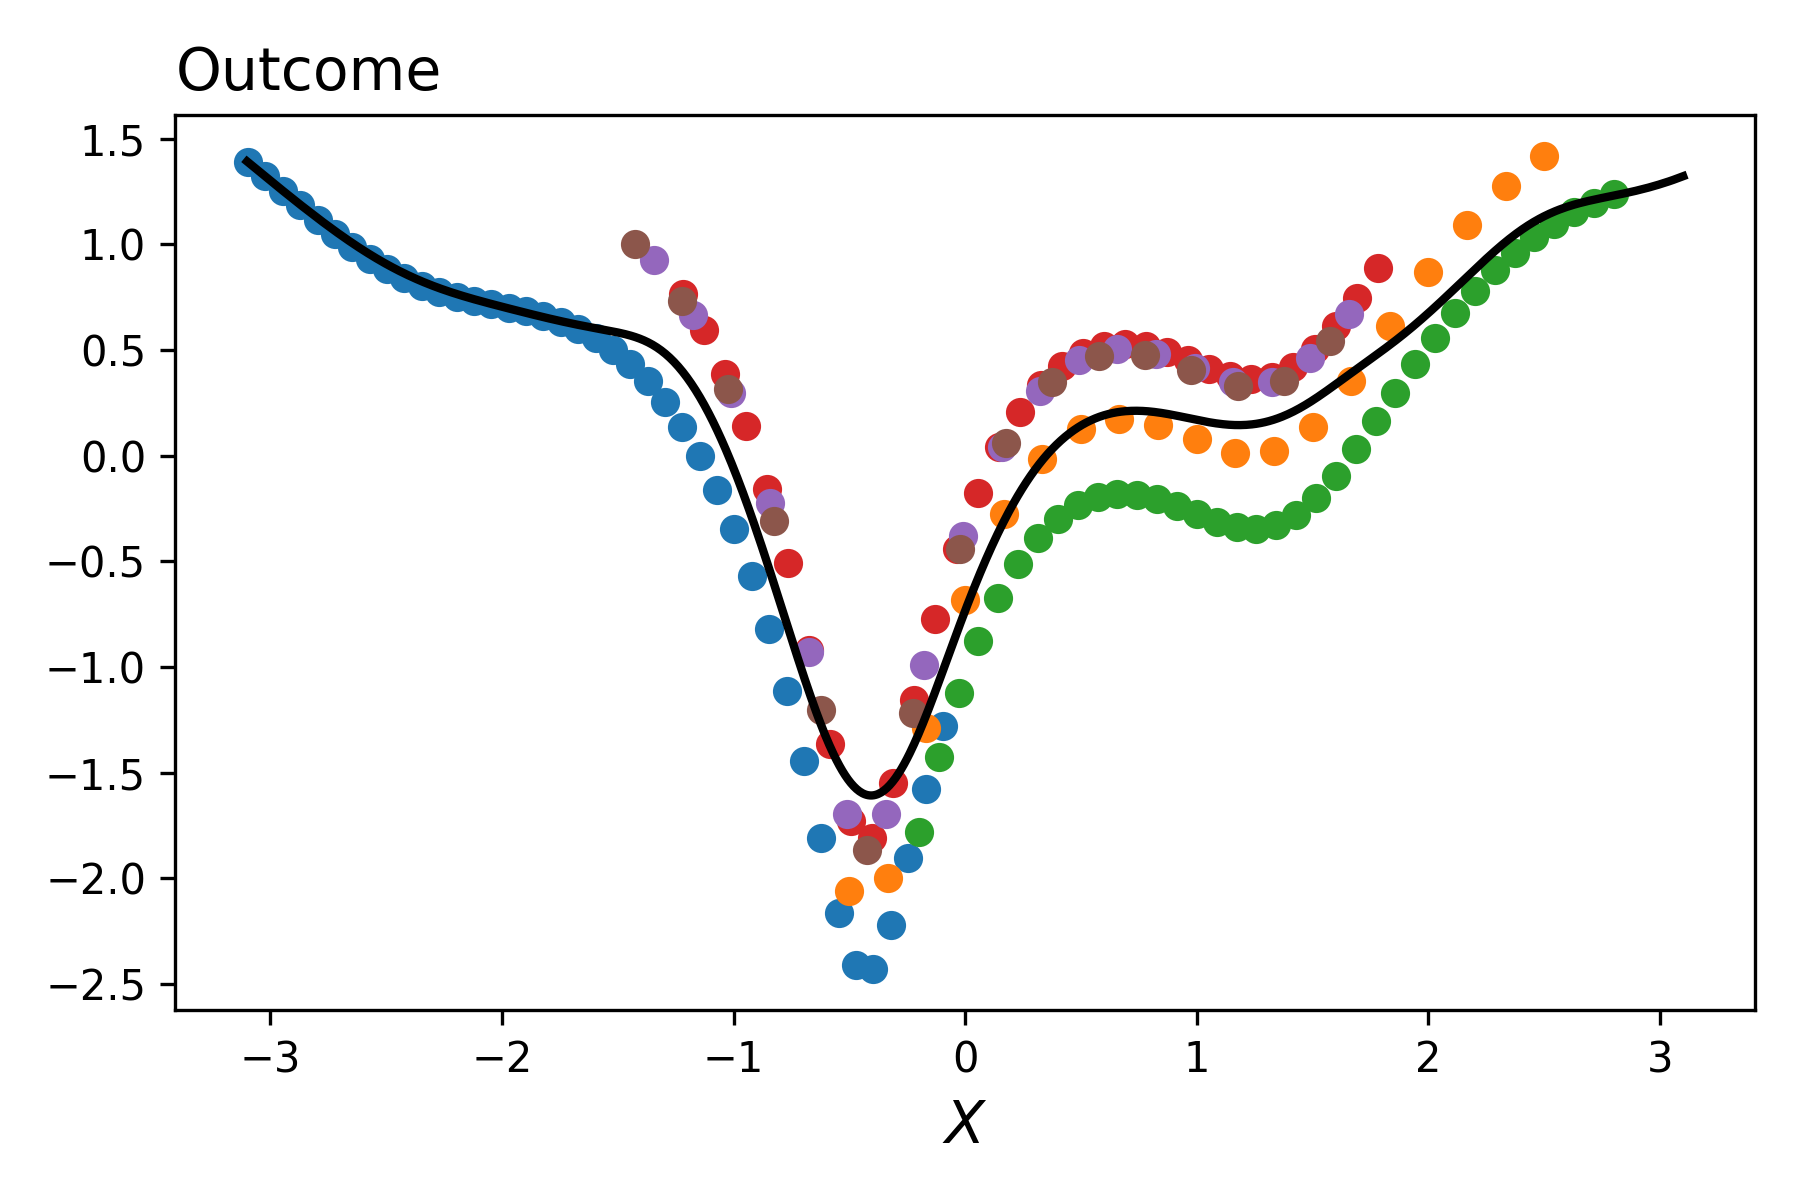
\includegraphics[scale=0.3]{figures/framework/local_linear_no_const_5.0_18_LM.png}
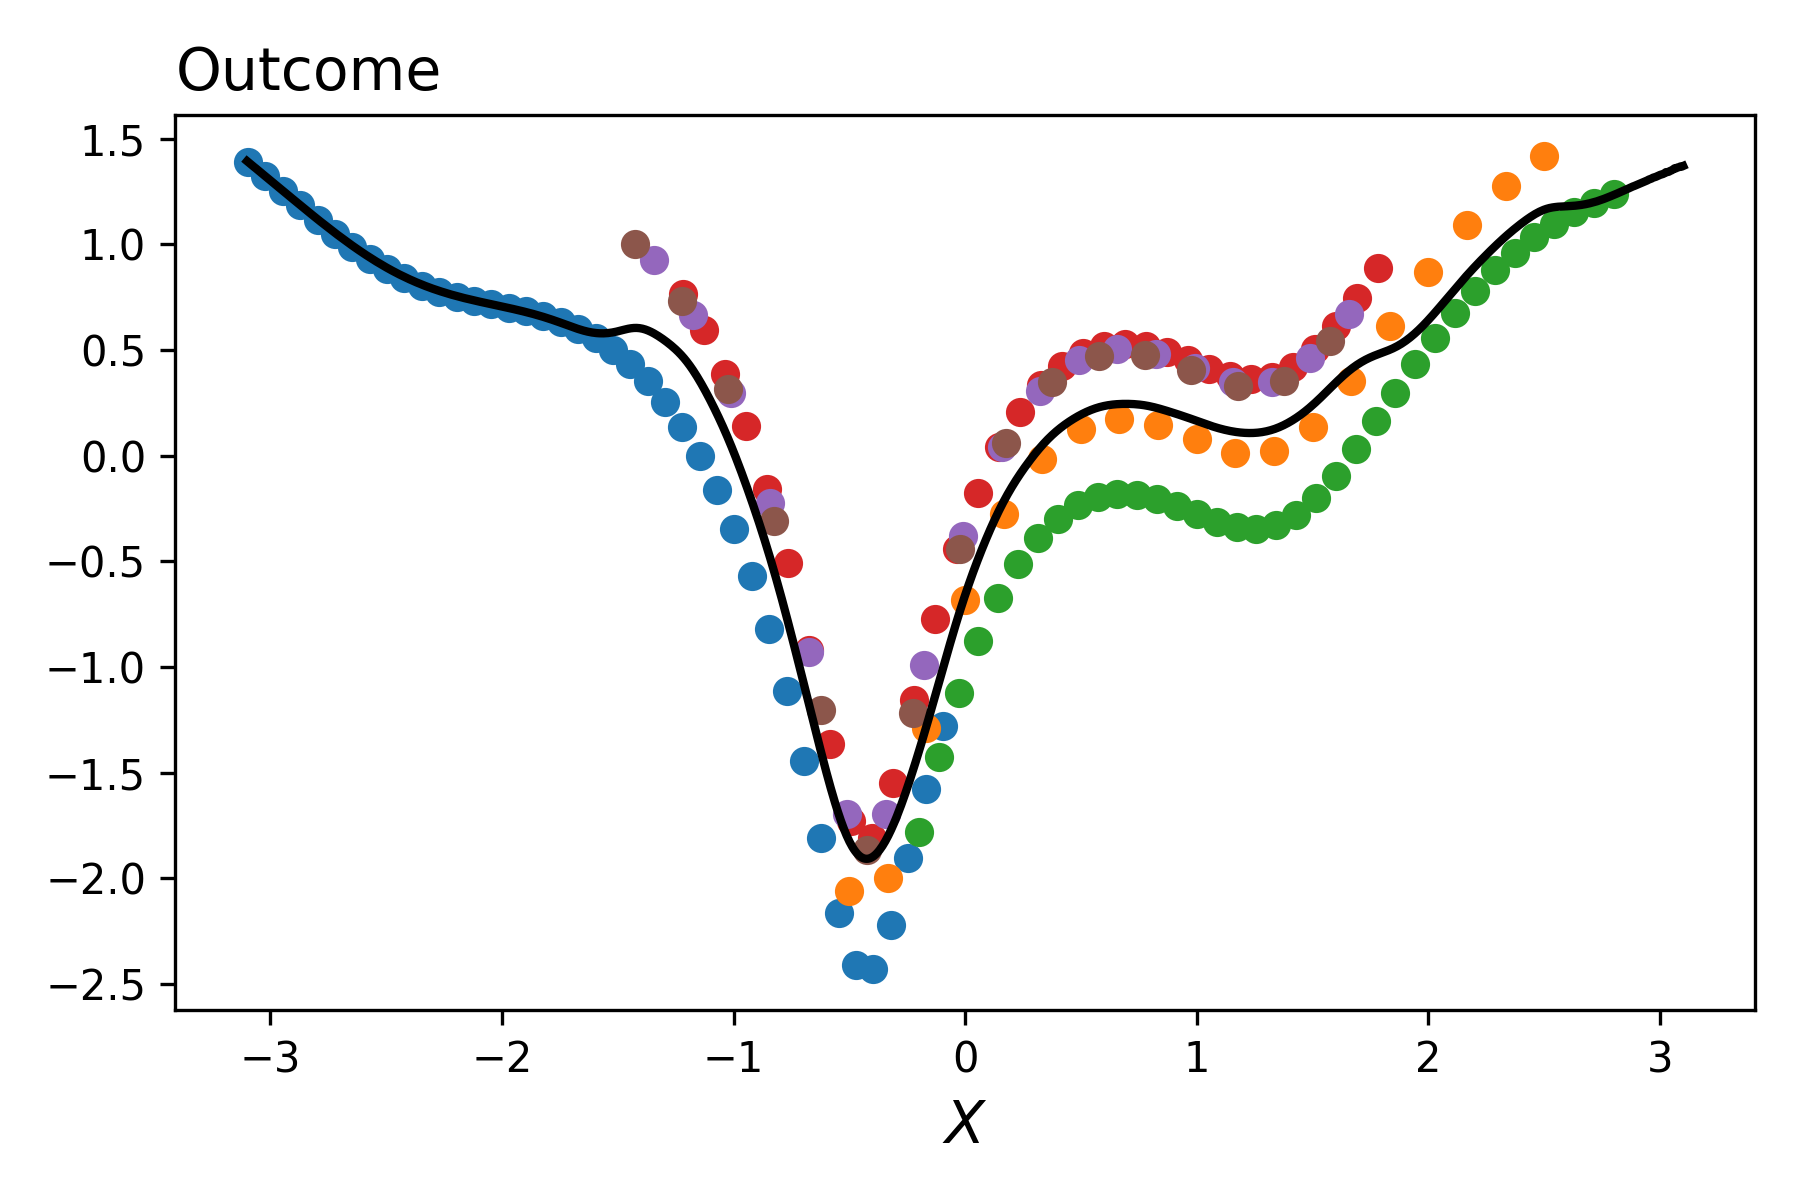
\includegraphics[scale=0.3]{figures/framework/local_linear_no_const_10.0_18_LM.png}
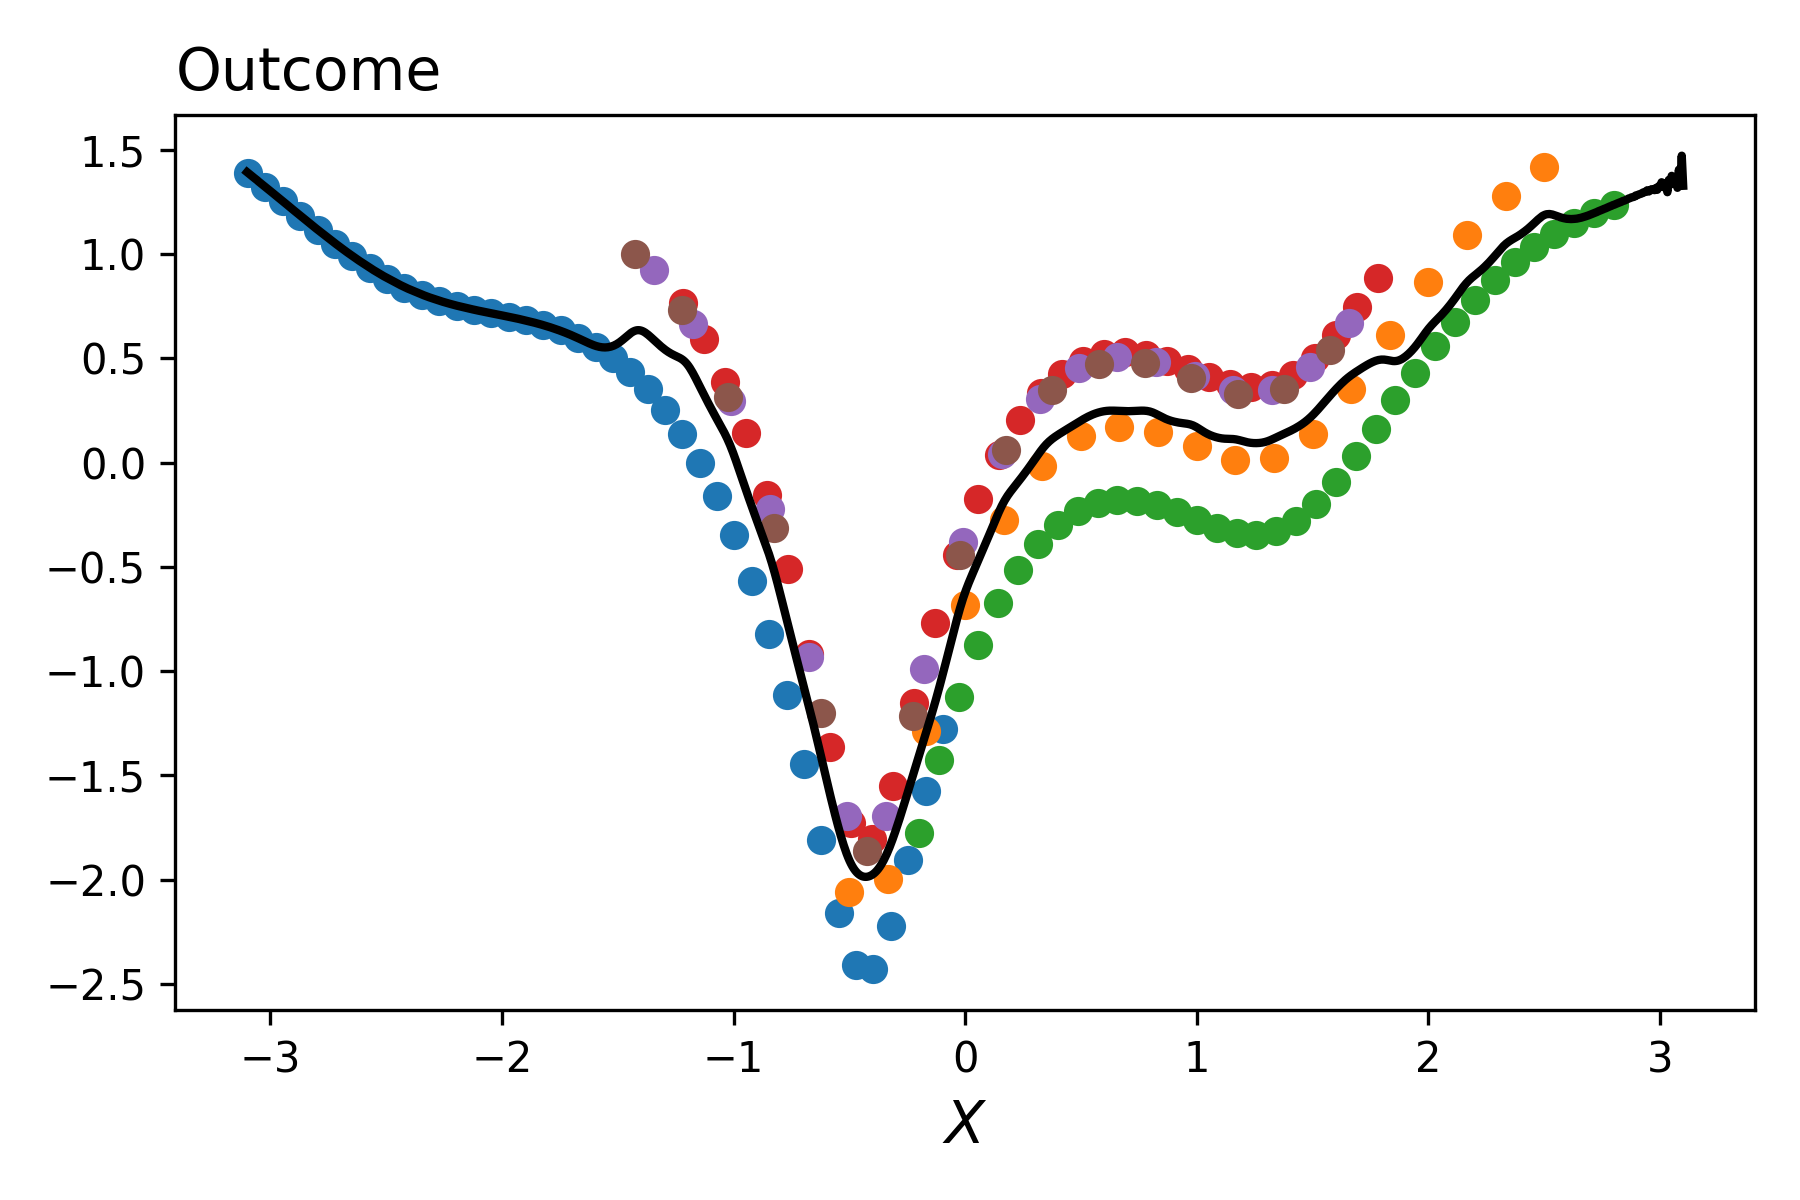
\includegraphics[scale=0.3]{figures/framework/local_linear_no_const_15.0_18_LM.png}
\caption{The general pattern that these figures try to highlight is that in order to fit the the `v`-shaped valley in the function, the model overfits the tails of the function -- \href{https://github.com/pharringtonp19/rfp/blob/main/notebooks/local_weighted_linear_regression_no_avg_effect_LM.ipynb}{Reproduced Here}}
\label{fig:nonparametrics}
\end{figure}
In contrast, subject to the appropriate hyperparameters, our method produces a reasonable estimate.

\begin{figure}[htbp]
\centering
\begin{subfigure}{.48\textwidth}
    \centering
    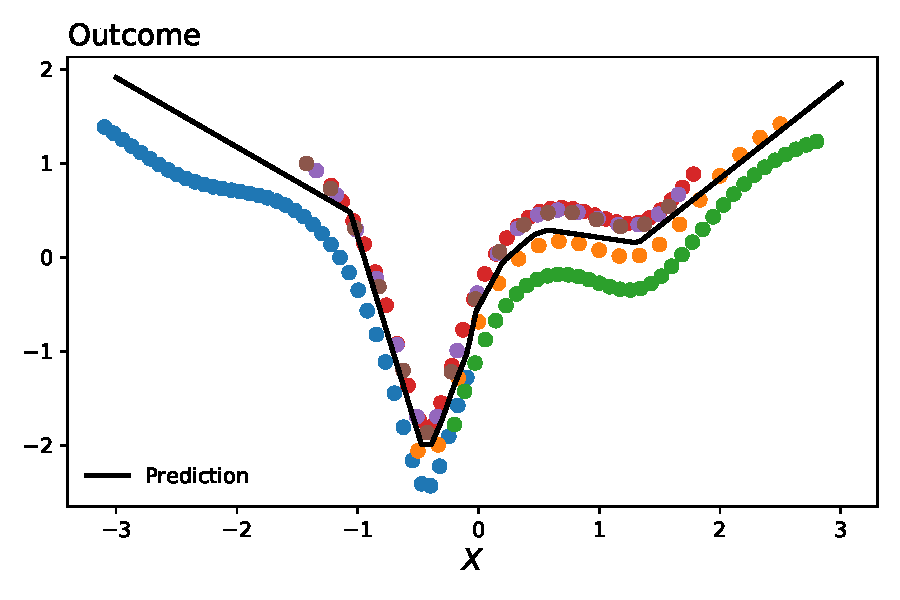
\includegraphics[width=.95\linewidth]{figures/framework/gradient_descent_motivating_example.pdf}
    %\caption{All zip codes}
    %\label{SUBFIGURE LABEL 3}
\end{subfigure}
\begin{subfigure}{.48\textwidth}
    \centering
    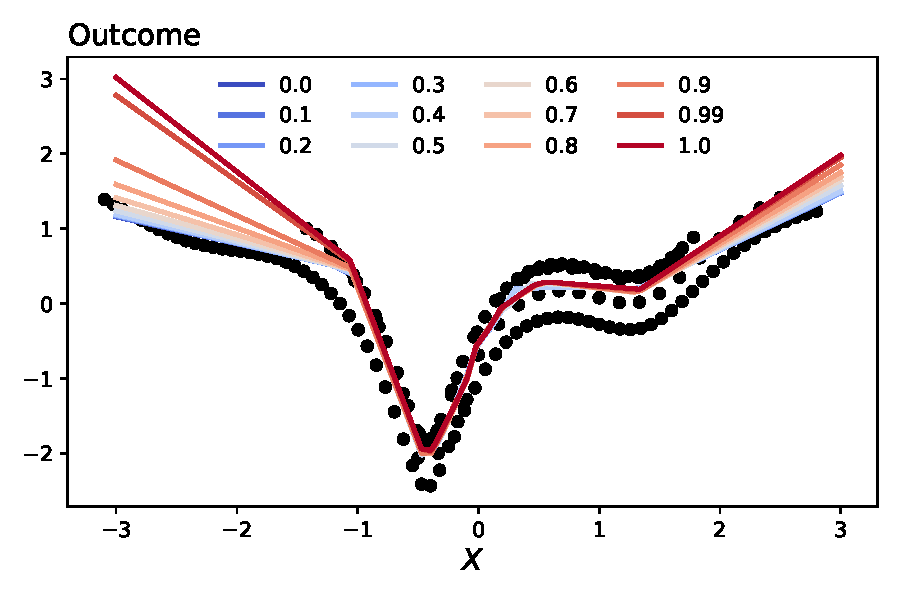
\includegraphics[width=.95\linewidth]{figures/framework/gradient_descent_motivating_example_tune.pdf}
    %\caption{High Eviction Zip Codes}
    %\label{SUBFIGURE LABEL 4}
\end{subfigure}
\caption{The general pattern that these figures try to highlight is that in order to fit the the `v`-shaped valley in the function, the model overfits the tails of the function -- \href{https://github.com/pharringtonp19/jmp_paper/blob/main/notebooks/gradient_descent_motivating_example.ipynb}{Reproduced Here}}
%\label{FIGURE LABEL}
\end{figure}
\subsection{Implicit Cluster Map}
\textbf{TL;DR} In this section, we define our implicit cluster map as a regularized version of the popular gradient based meta-learning MAML.\footnote{Model Agnostic Meta-Learning (MAML), a method that consists of two optimization loops, with the outer loop finding a meta-initialization,
from which the inner loop can efficiently learn new tasks.-- \cite{raghu2019rapid}} While follow-up work such as \cite{raghu2019rapid} has shown that the ``the meta-initialization already providing high quality
representations'', such an analysis assumes a cluster specific head of the network. We show that empirically, without this cluster specific head, the meta-initialization is not done in the right space which motivates our need to add an additional form of regularization.

As applied microeconomists, we are accustomed to writing our problem as a bi-level optimization problem so as to better distinguish between the parameters of interest and the nuisance parameters. In this context, the nuisance parameters are cluster specific parameters that are ``fit'' during the inner optimization process. Below, we follow the language used by \cite{belkin2021fit} in distinguishing between classical and modern estimation techniques.
 
\begin{align*}
    \mathcal{L}(\theta) &:= \sum _c \mathcal{L}_c(\theta), \quad \mathcal{L}_c(\theta) := G(\theta, \theta^*_c(\theta)), \quad  \theta_c^*(\theta) := \underset{\theta_c}{\textrm{argmin}} \ F(\theta, \theta_c) 
\end{align*}

With “Classical” under-parameterized models, as in the case of linear regression, $F$, the clustere-specific empirical loss function is exactly what you would expect. 
\begin{align*}
    F(\theta, \theta_c^*(\theta)) := \sum _{i \in c}\big(y_i - \theta^Td_i - \theta _c^*(\theta)^Tx_i \big)^2
\end{align*}
 With“Modern” over-parameterized models, though, like the ones that we target in this paper, we make the following adjustments. 
 We restrict the objective function that is used to implicitly define the cluster specific maps. First, we generalize the above set-up by allowing the cluster specific parameters to be in one-to-one correspondance with the parameters of interest. Second, we constrain the implicit cluster function $\theta_c^*(\theta)$. Without some form of regularisation, given the flexibility of neural network models as illustrated in \cite{zhang2021understanding}, the jacobian of this function can easily be zero. We illustrate this concern in figure \ref{fig:Missinggrads}. And finally, we add a penalty term to the cluster specific loss function to ensure that adaptation happens in the right space. 
 

\begin{align*}
\intertext{Define our empirical cluster parameters in relation to the parameters of interest}
    G(\theta) &:= \sum _{i \in c}\big(y_i - f(\theta_c^*(\theta), x_i)\big)^2
\intertext{Implicit Cluster Map}
\theta_c^*(\theta) &:= \theta^t - \alpha \nabla_{\theta}G(\theta^{t-1}), \quad \theta^{0} = \theta 
\intertext{As well as introduce an auxilliary term to the cluster specific loss function}
    \mathcal{L}_{c}(\theta) &:= G(\theta) + H(\textrm{Path}(\theta, \hat{\theta}^*_c(\theta)))
\end{align*}
We illustrate the relative importance of our design choices in figure \ref{fig:mamlablation}. In figure \ref{fig:overfittails} we see that supverized learning overfits to the clusters in the tails of their distributions. In figure \ref{fig:wrongspace}, we see that MAML meta initialization is in the wrong space. And finally in figure \ref{fig:rfp}, we see that a regularized version of MAML appears to learn something reasonable. 
\begin{figure}[htbp]
\centering
\begin{subfigure}{.32\textwidth}
    \centering
    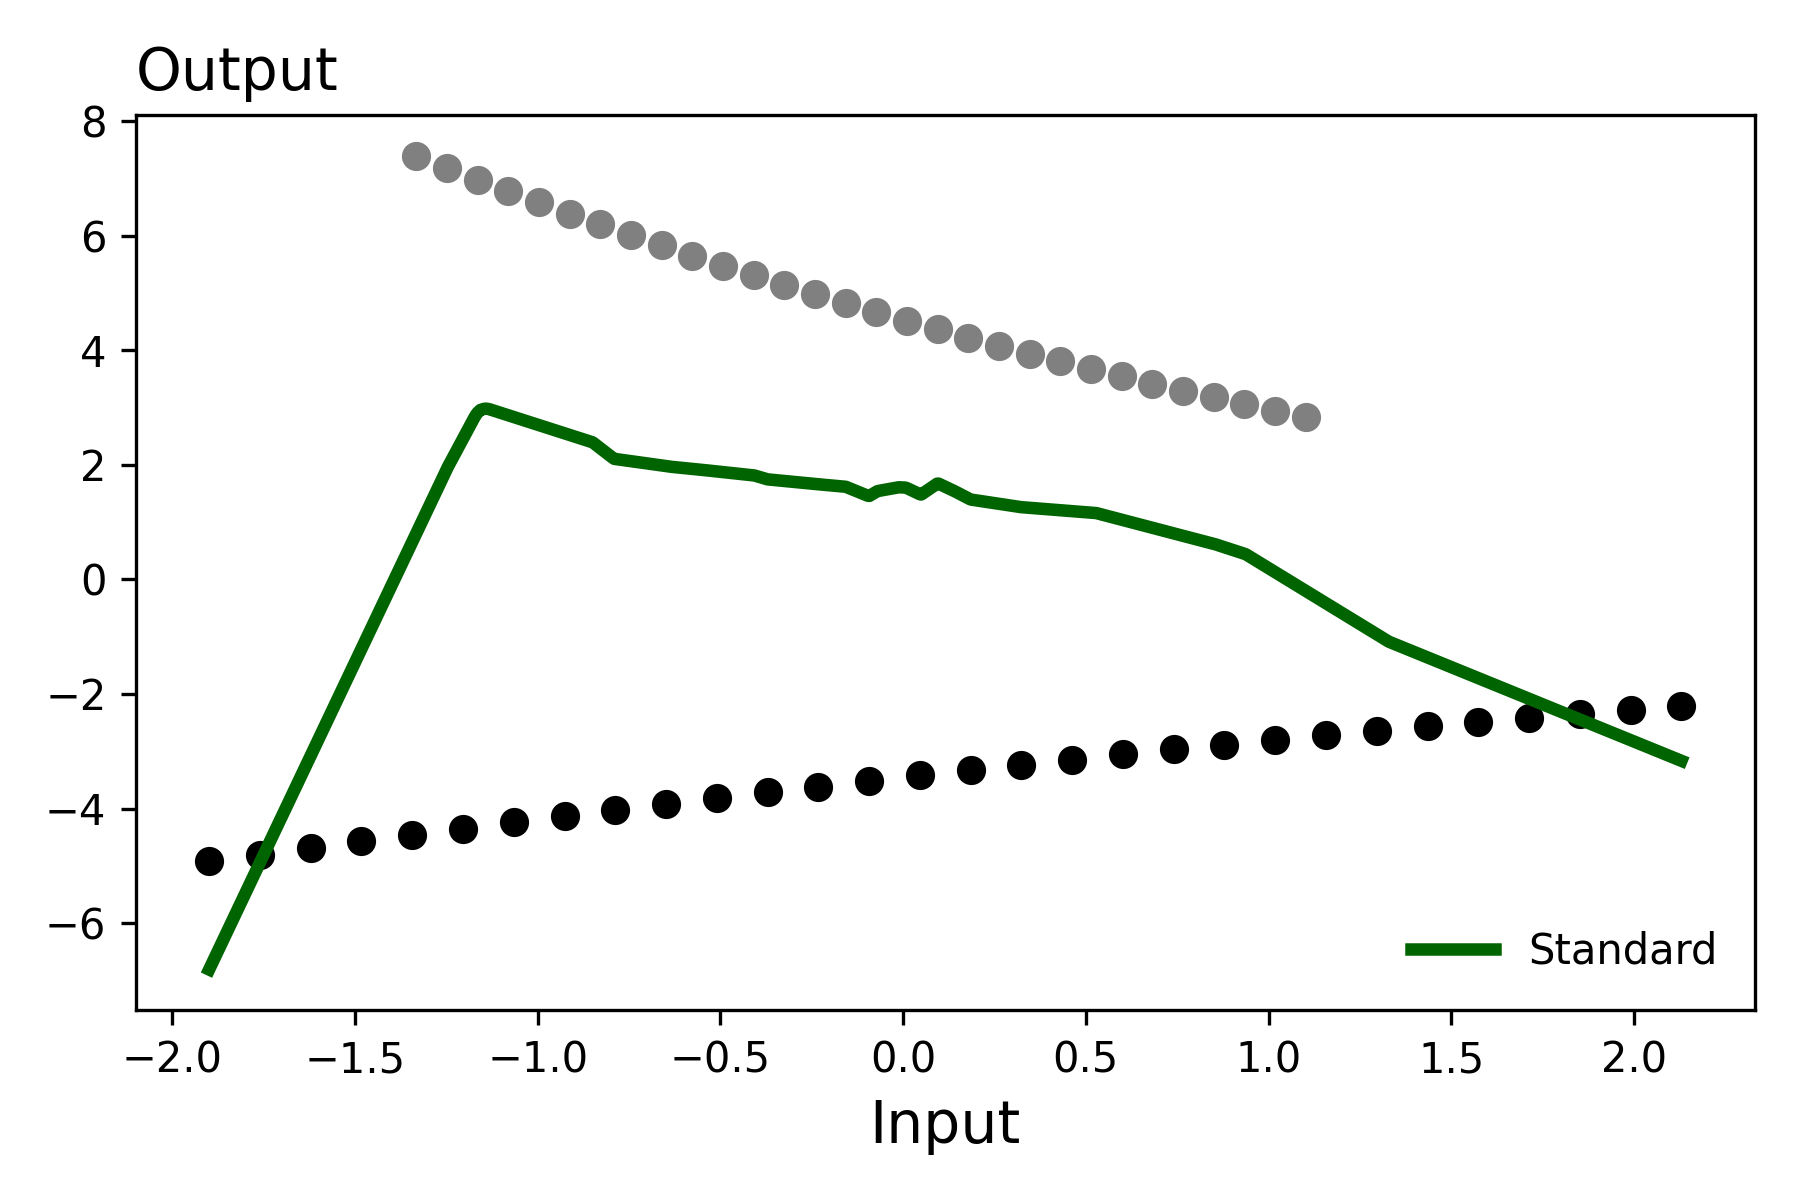
\includegraphics[width=.95\linewidth]{figures/framework/grad_desc_toy_Standard.png}
    \caption{Standard Training}
    \label{fig:overfittails}
\end{subfigure}
\begin{subfigure}{.32\textwidth}
    \centering
    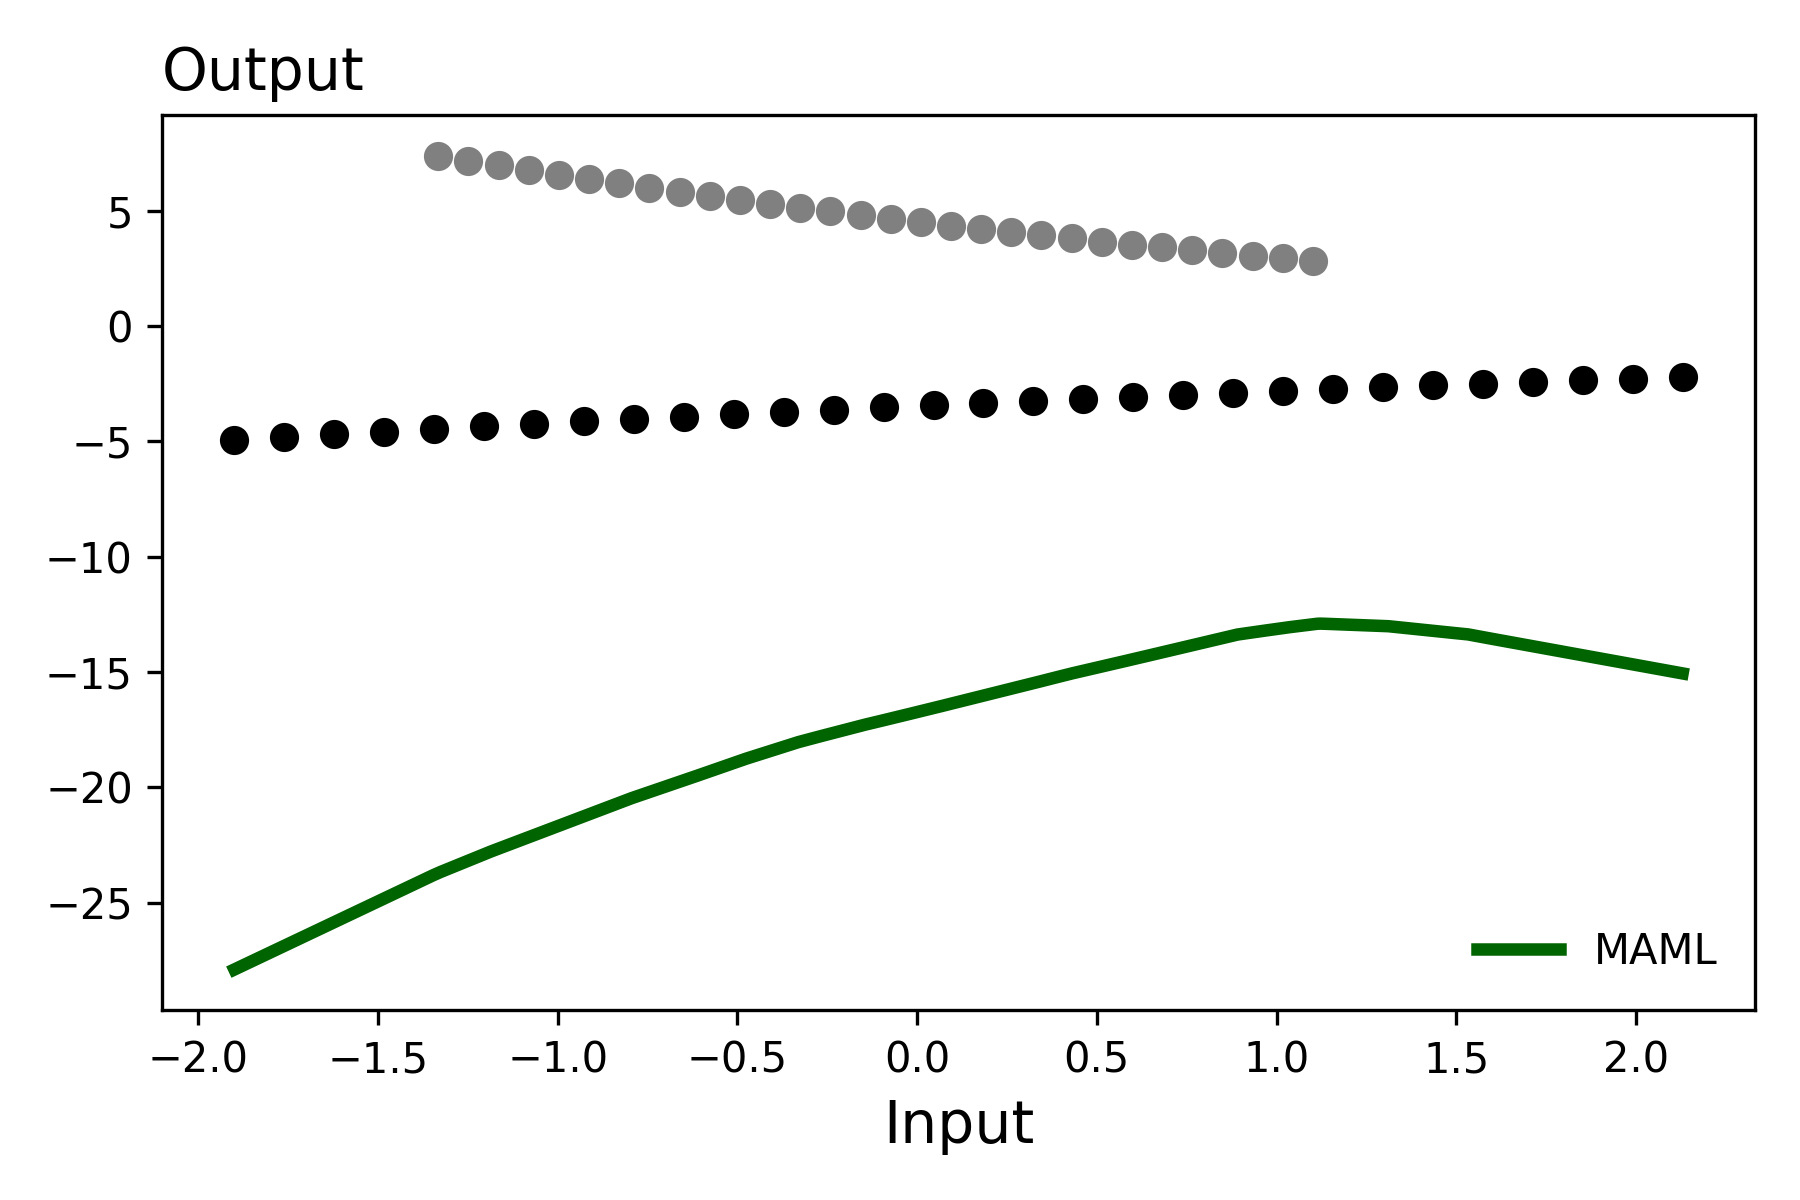
\includegraphics[width=.95\linewidth]{figures/framework/grad_desc_toy_MAML.png}
        \caption{MAML}
    \label{fig:wrongspace}
\end{subfigure}
\begin{subfigure}{.32\textwidth}
    \centering
    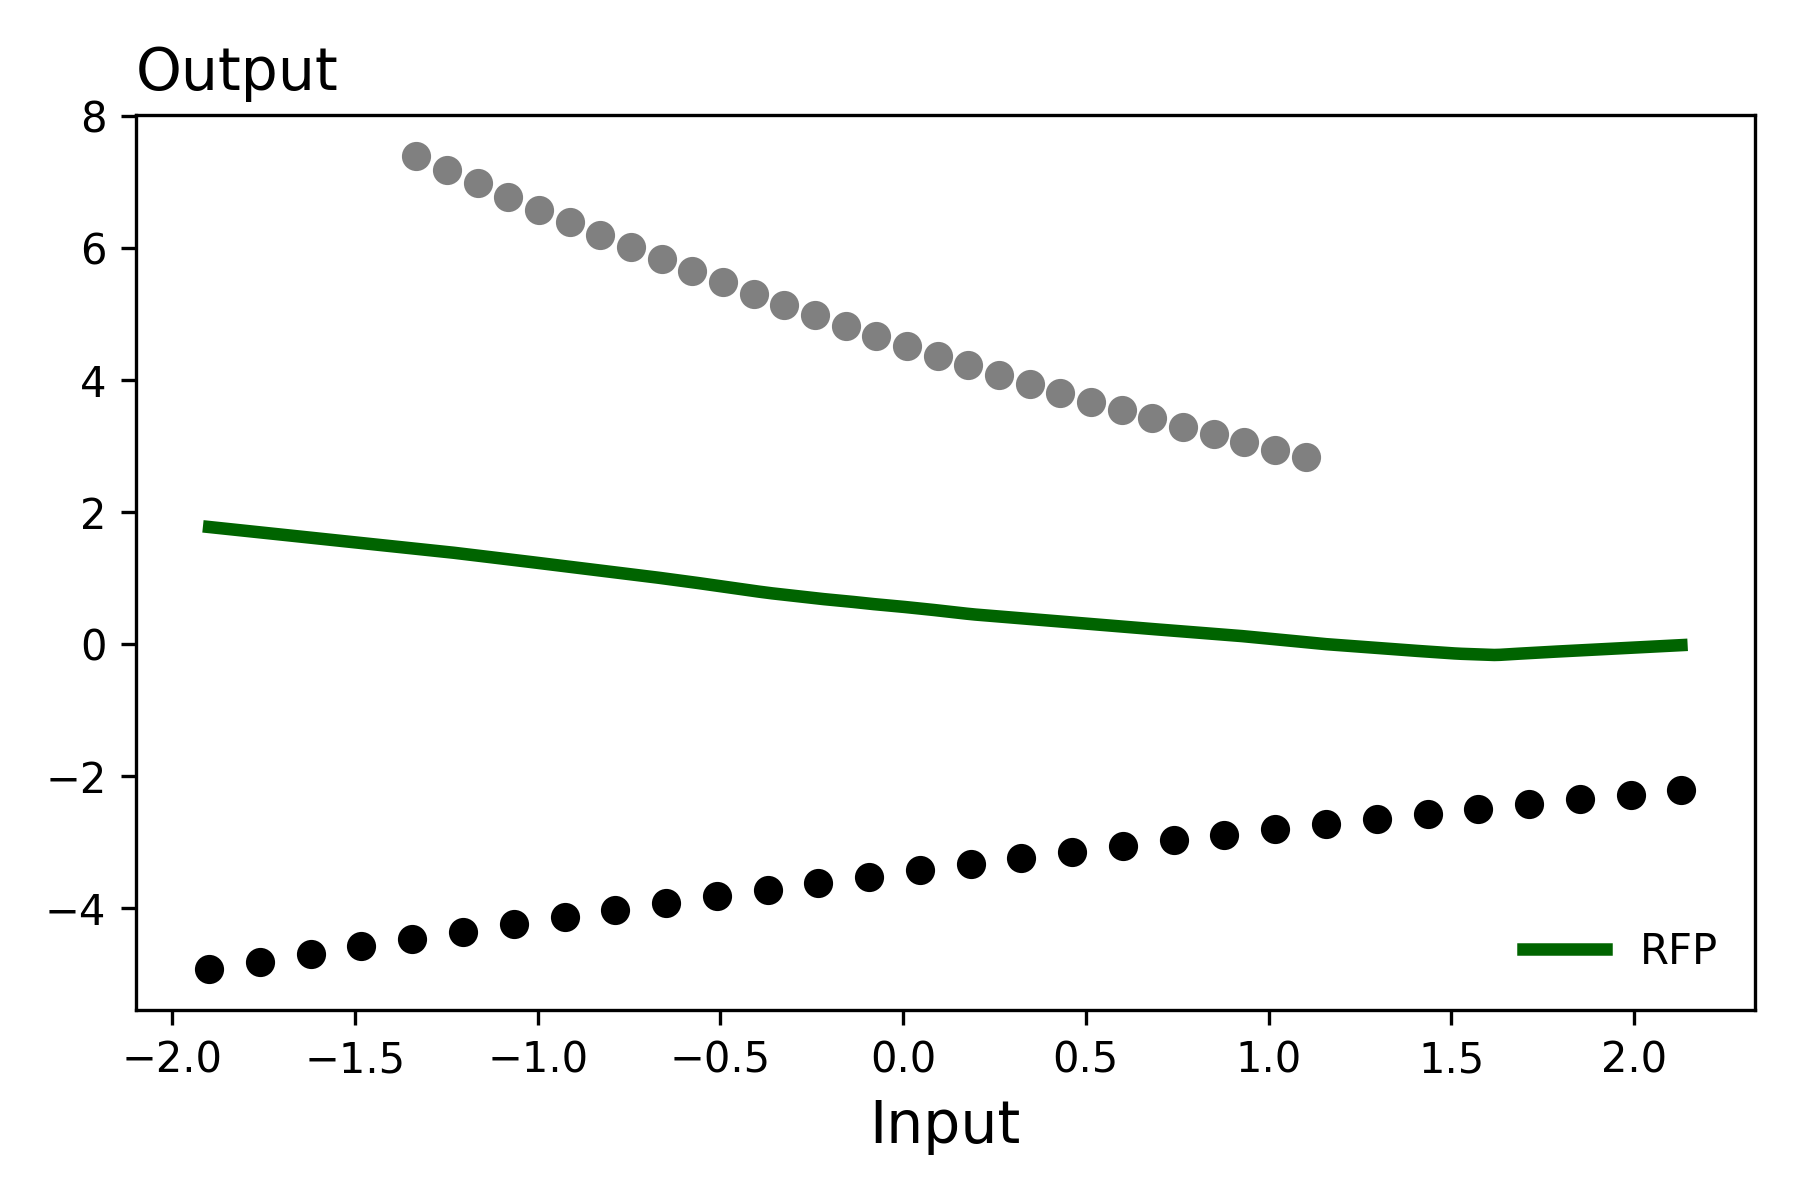
\includegraphics[width=.95\linewidth]{figures/framework/grad_desc_toy_RFP.png}
        \caption{RFP}
    \label{fig:rfp}
\end{subfigure}
\caption{ \href{https://github.com/pharringtonp19/rfp/blob/main/notebooks/grad_desc_toy.ipynb}{Reproduced Here}: The grey and black dots represent data from separate clusters. Each figure corresponds to fitting a neural network to this data under different training algorithms}
\label{fig:mamlablation}
\end{figure}


\section{Toy Model}
\subsection{Overview}
In order to clarify our estimand of interest, we write down the following model. The key detail is that we parameterize the constraint function with the Right to Counsel Policy. Everything else is rather standard in that we allow the parameters of the constraint and utility functions to differ across individuals, and define our estimand as the expected value take with respect to these the probability law induced by these random variables. \textbf{Notationally}, we denote the partial evaluation of a function by subscripting the function with the argument.\par 
\subsection{Model}
We define an element of the choice set as a bundle of housing related features. Most relevant to our data set is the housing search length which we include as the first component. It's important to acknowledge that individuals may be substituting across a wide range of housing aspects including the quality of the house and the price among others features.\footnote{To introduce uncertainty into the model, we could augment each housing bundle with a stochastic process that captures the probability of remaining in the house across each time period. Note, this stochastic process would likely vary across individuals.}
\begin{align*}
    x := (\textrm{search period}, \textrm{quality}, \textrm{price}, \dots ) \in \mathcal{X}
\end{align*}
As indicated by its signature, we introduce a parameterized constraint function where we allow the parameters to vary across individuals. This constraint function not only incorporates the macroeconomic features of the housing market, but also the landlords actions/policies towards individual tenants.
\begin{align*}
   F :: \textrm{Params} \to  \textrm{RTC} \to \mathcal{X} \to \{0, 1\} 
\end{align*}
The uttility function then captures some (present discounted) value of each housing option. 
\begin{align*}
U :: \textrm{Params} \to \mathcal{X} \to \mathcal{R}_+ 
\end{align*}
With the essential components of the model defined, we can express the individual choice problem as follows. The following problem would model an individual not in a treated zip code or prior to the policy implementation as the second parameter of the constraint function takes the value $0$. The pre-image of $0$ under the constraint function defines the feasibility set. 
\begin{align*}
\underset{x \in F_{p, 0}^{-1}(0)}{\textrm{maximize}} \ U_{\alpha} (x)
\end{align*}
Via-this parameterized optimization problem, we can then define the implicit function of interest which captures the effects of the individual-level parameters and the policy on the search length. 
\begin{align*}
s^*(\textrm{rtc}, p, \alpha) := \underset{x \in F_{p, \textrm{rtc}}^{-1}(0)}{\textrm{argmax}_0} \ U_{\alpha} (x) \\ 
\end{align*}
As we are only interested in the later effects, we integrate over the individual-level parameters leading to the estimand defined below.
\begin{align*}
&\theta := \mathbb{E}[s^*(1, p, \alpha) - s^*(0,  p, \alpha)] \\
&\quad = \int _{\Omega} s^*\big(1, p(\omega), \alpha(\omega)\big) - s^*\big(0, p(\omega), \alpha(\omega)\big)d\mathbb{P}
\end{align*}

 




\section{Empirical Strategy}
The following notation defines the key variables used in the estimators defined below. 
\begin{align*}
    &Y_i:  \textrm{Search Duration}\\
    &X_i: \textrm{Age, Gender, Race, Family Size}\\ 
    %&P_i: \textrm{Rapid Rehousing Provider}\\ 
    &Z_i: \textrm{Zip Code} \\
    &D_i: \textrm{Treated Zip Code}
\end{align*}
\textbf{Note}: Subscripts on the outcome corresponding to subsets of individuals who are observed in that corresponding time period. 

\subsection{Difference-in-Difference}
We fit the following difference-in-difference estimator. In this specification and for the ones that follow, $Y_i$ is a binary variable that indicates whether the search length was less than some specified number of days. As we illustrate in figure \ref{fig:diff_mean}, the percentage point effect of the Right to Counsel (the y-axis) is relatively consistent as we vary the acceptable move-in-date threshold. 
\begin{align*}
    \beta_0 &= \mathbb{E}[Y_1 -Y_0 \mid D=1] -  \mathbb{E}[Y_1 - Y_0 \mid D=0] \end{align*}
Importantly, when we restrict the sample to only high eviction zip codes in figure \ref{fig:diff_mean_high}, we see a relatively consistent negative effect on the probability of moving into housing by a certain date.
\begin{figure}[htbp]
\centering
\begin{subfigure}{.48\textwidth}
    \centering
    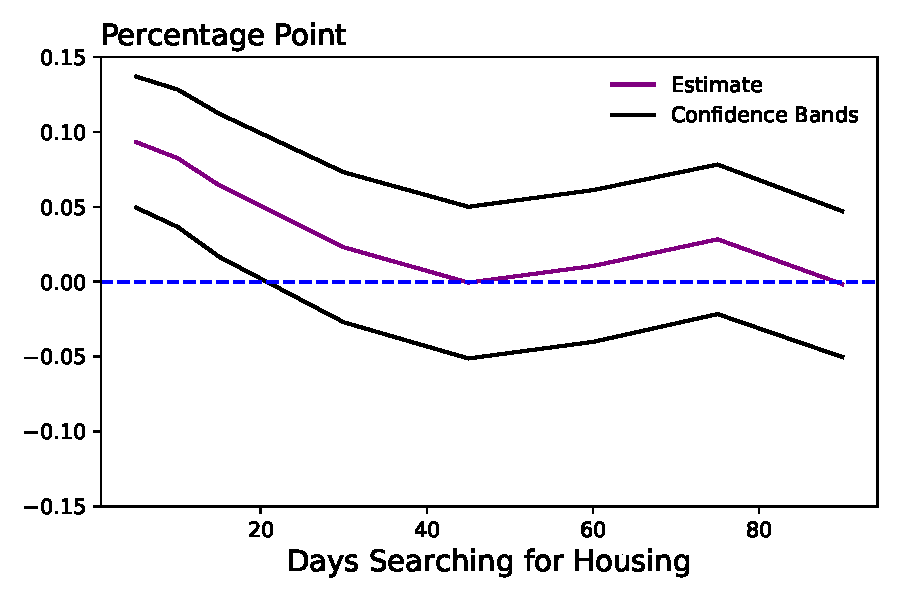
\includegraphics[width=.95\linewidth]{figures/rtc/results/cceh/diff_in_mean_False_False.pdf}
    \caption{All zip codes}
    \label{SUBFIGURE LABEL 3}
\end{subfigure}
\begin{subfigure}{.48\textwidth}
    \centering
    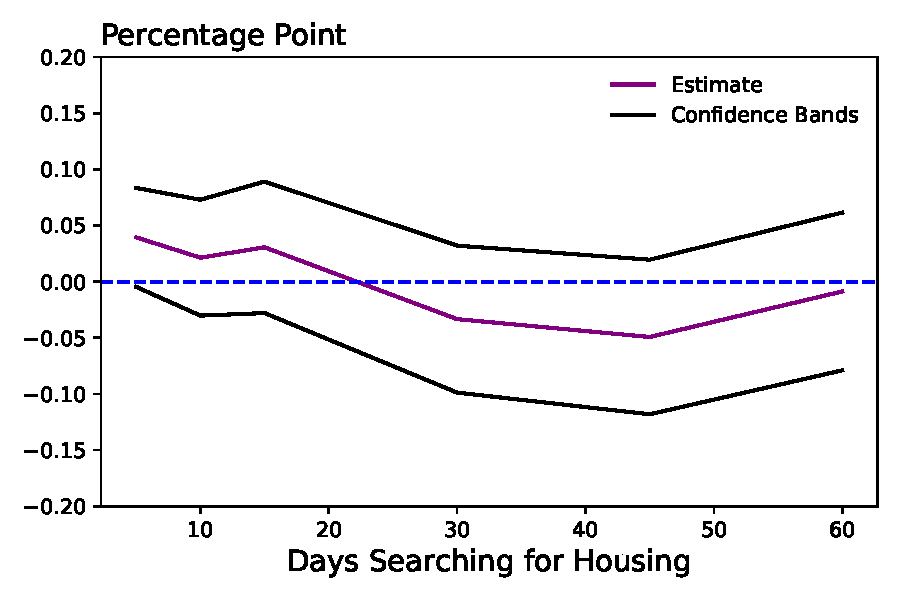
\includegraphics[width=.95\linewidth]{figures/rtc/results/cceh/diff_in_mean_True_False.pdf}
    \caption{High Eviction Zip Codes}
    \label{fig:diff_mean_high}
\end{subfigure}
\caption{ \href{https://github.com/pharringtonp19/evictions/blob/main/scripts/cceh/primary/diff_n_mean_rrh.py}{Reproduced Here}: Confidence Bands formed via stratified bootstrapped sampling without replacement (75\%)}
\label{fig:diff_mean}
\end{figure}

\subsection{Difference-in-Difference with Controls}
Adding individual level controls as well as zip code fixed effects makes a material difference for the magnitude of the effect but not the sign when we again restrict the sample to high eviction zip codes in figure \ref{fig:diff_control_high}.
\begin{align*}
    Y_i &= \alpha _0 + \beta_0 \textrm{Post}_i \times \textrm{Treated}_i + \beta_1  \textrm{Post}_i + \beta_2 \textrm{Treated}_i \\ 
    &\quad + \beta _3X_i + \beta_4 Z_i + \varepsilon_i
\end{align*}
\begin{figure}[htbp]
\centering
\begin{subfigure}{.48\textwidth}
    \centering
    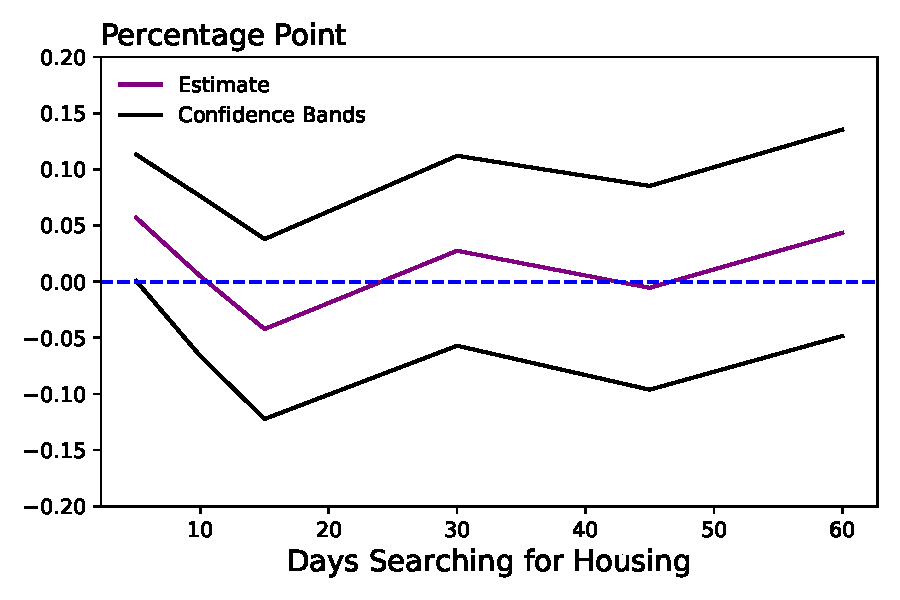
\includegraphics[width=.95\linewidth]{figures/rtc/results/cceh/linear_reg_False_False.pdf}
    \caption{All zip codes}
    \label{SUBFIGURE LABEL 3}
\end{subfigure}
\begin{subfigure}{.48\textwidth}
    \centering
    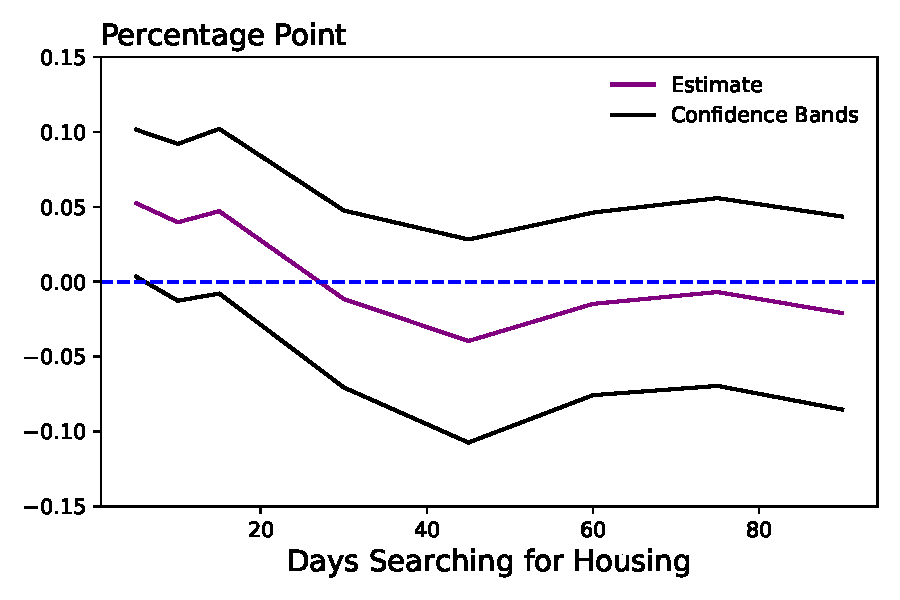
\includegraphics[width=.95\linewidth]{figures/rtc/results/cceh/linear_reg_True_False.pdf}
    \caption{High Eviction Zip Codes}
\label{fig:diff_control_high}
\end{subfigure}
\caption{ \href{https://github.com/pharringtonp19/evictions/blob/main/scripts/cceh/primary/diff_n_mean_rrh.py}{Reproduced Here}: Confidence Bands formed via stratified bootstrapped sampling without replacement (75\%)}
\label{fig:diff_control}
\end{figure}

%\subsection{Partially Linear Difference-in-Difference}

\subsection{Regularizing the Forward Pass}
It's possible to re-write the difference-in-difference model with controls as a linear version of the following estimator. Doing to we see that there are two potential concerns. The first is that the model fails to correct for the propensity score which as highlighted in figure \ref{fig:DML} can be problematic in certain contexts.  

\begin{align*}
\tilde{Y}_i - \mathbb{E}[ \tilde{Y}_i | X_i] = \beta_0 \big(D_i - \mathbb{E}[D_i |X_i]\big) + \varepsilon_i, \quad \textrm{where} \ \tilde{Y}_i =  Y_{1i} - Y_{0i} 
\end{align*}

\begin{figure}[htbp]
\centering
\begin{subfigure}{.48\textwidth}
    \centering
    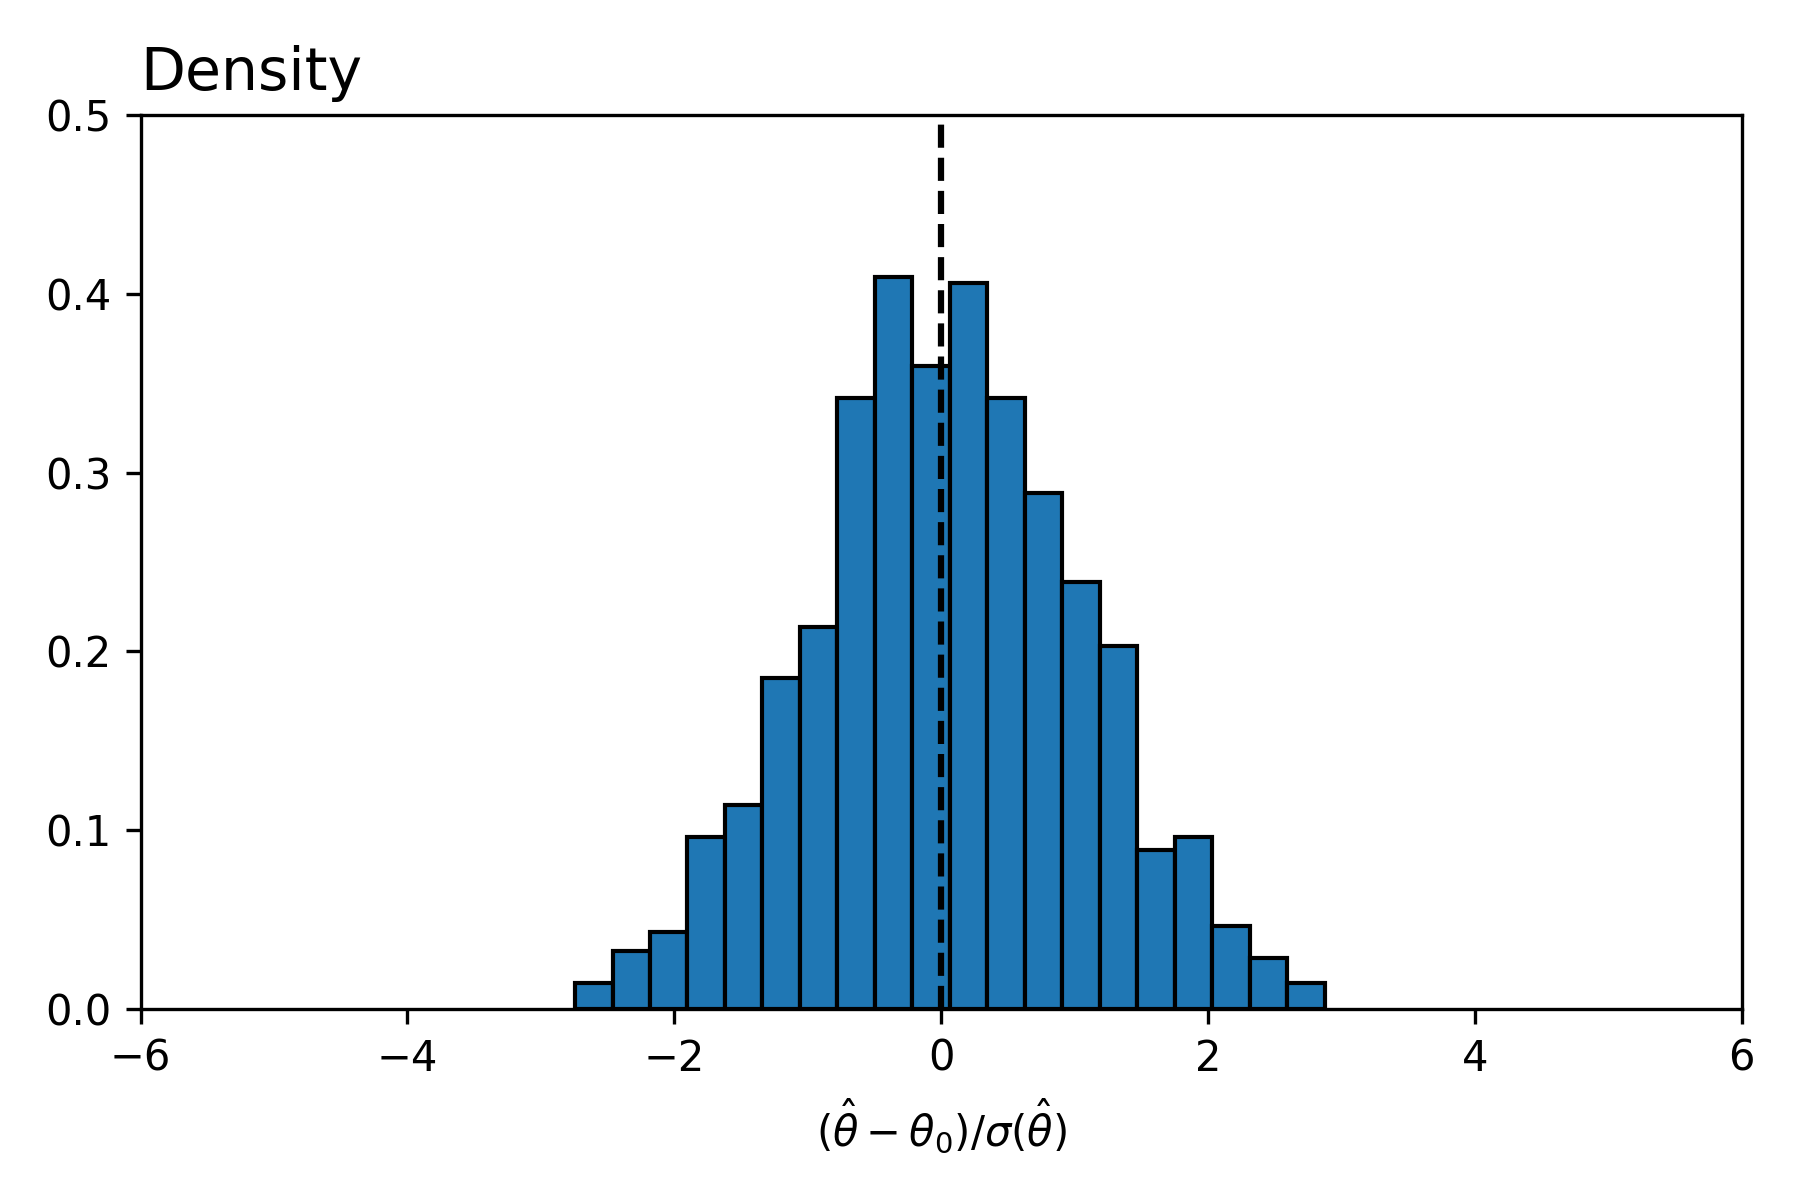
\includegraphics[width=.95\linewidth]{figures/framework/dml_True.png}
    \caption{Original Paper}
    %\label{SUBFIGURE LABEL 3}
\end{subfigure}
\begin{subfigure}{.48\textwidth}
    \centering
    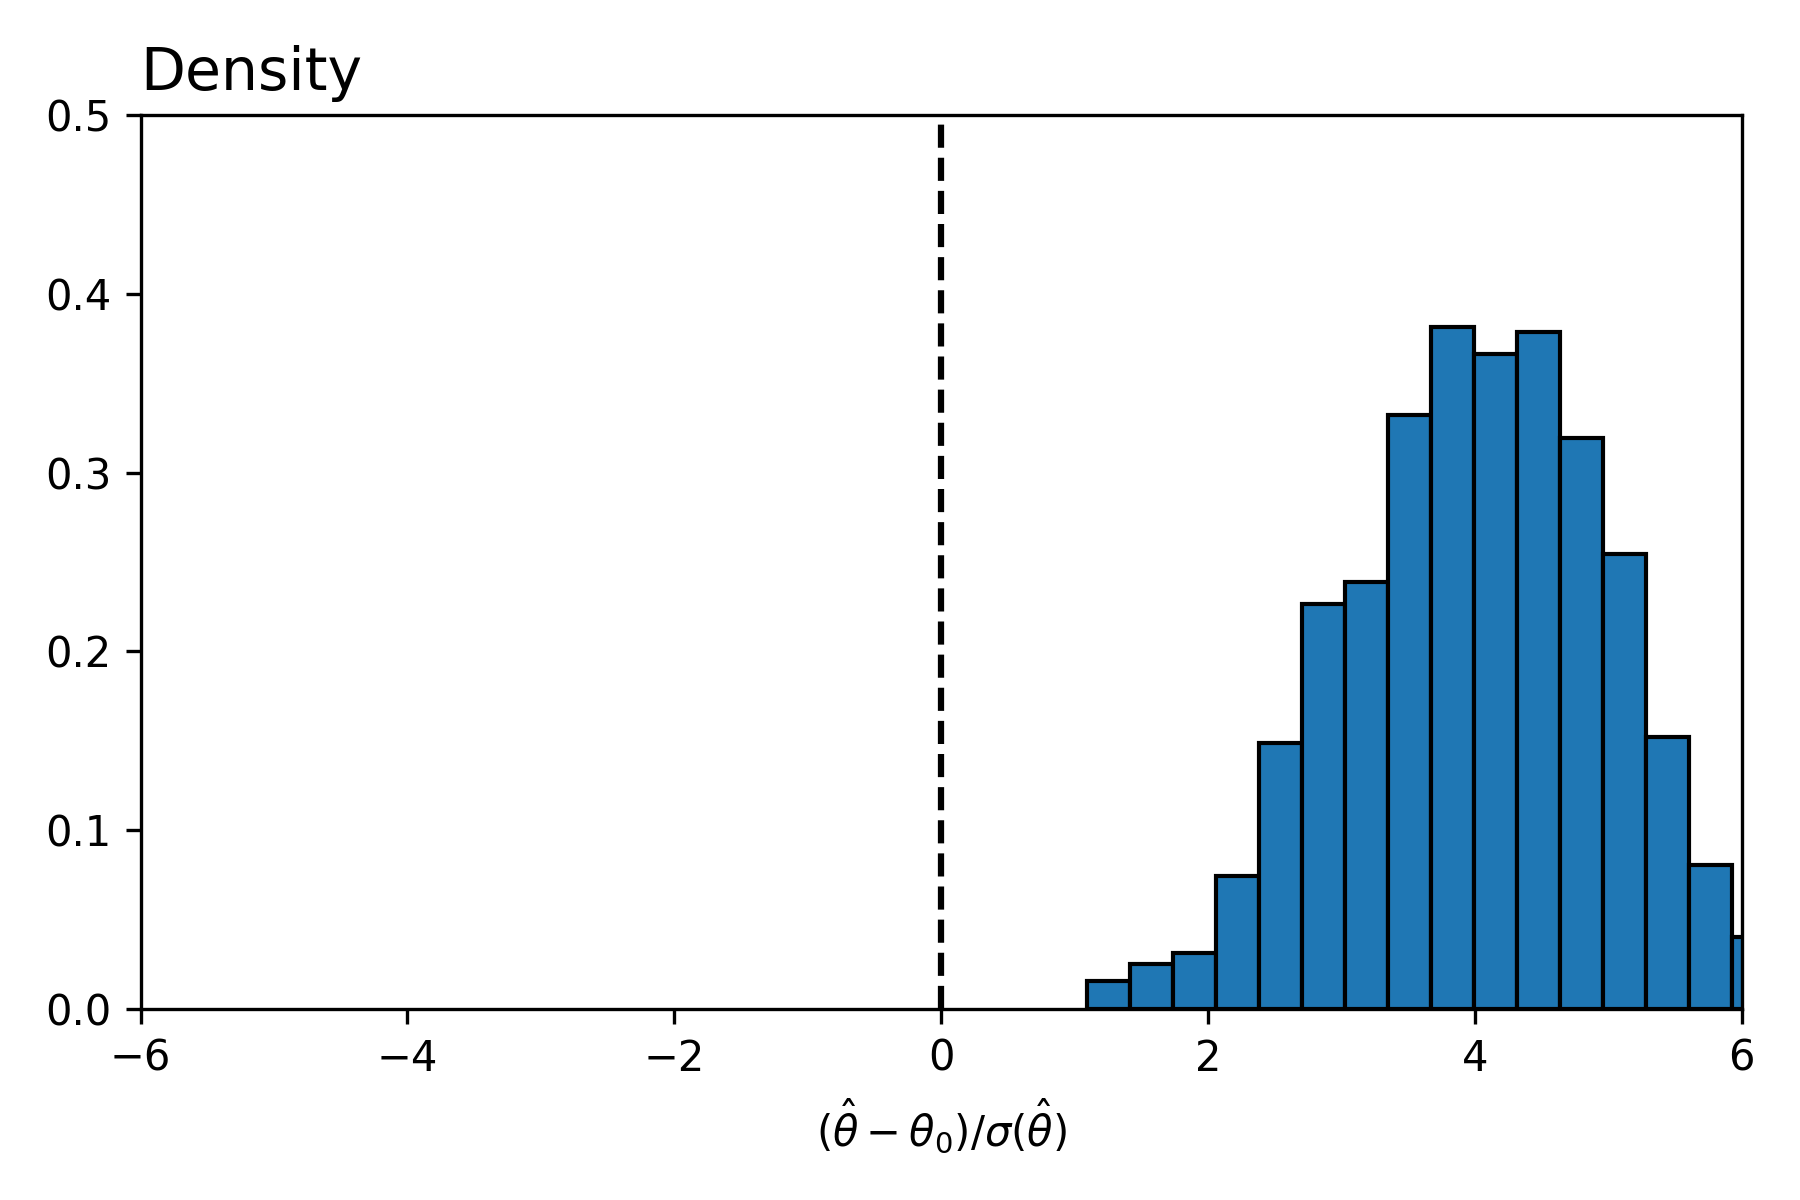
\includegraphics[width=.95\linewidth]{figures/framework/dml_False.png}
        \caption{Nonuniform Propensity Score}
    %\label{SUBFIGURE LABEL 4}
\end{subfigure}
\caption{ \href{https://github.com/pharringtonp19/rfp/blob/main/examples/scripts/dml.py}{Reproduced Here}: The sampling distribution of a Double Machine Learning Based Neural Network Estimator under selection on observables. In (a), we replicate the results of the original paper where the authors assume a constant treatment effect. Under a non-constant treatment effect as captured in (b), a failure to correct for the propensity score can introduce bias.}
\label{fig:DML}
\end{figure}
The natural correction is to then deploy a fully-nonparametric model. 
\begin{align*}
\beta_0 := \int \mathbb{E}[\tilde{Y}_i | X_i, D_i=1] - \mathbb{E}[\tilde{Y}_i | X_i, D_i=0] d\mathbb{P}_X
\end{align*}
As previously illustrated, though, when treatment varies at the cluster level such estimators are susceptible to the tragic triad. We therefore implicitly partiall out the cluster effects by fitting these conditional expectations using our regularized forward pass framework which generates the results captured in figure \ref{fig:rfp_results}. Note, in order to limit the computation burden of these models we fit the following model. The only difference is that it removes the first step of estimating $\tilde{Y}$. 

\begin{align*}
    \beta _0 := \int d\mathbb{P}_X\Big(\big(\mathbb{E}[Y_1 |X,D=1] - \mathbb{E}[Y_0 |X,D=1]\big) -  \big(\mathbb{E}[Y_1 |X,D=0] - \mathbb{E}[Y_0 |X,D=0]\big)\Big)
\end{align*}


\begin{figure}[htbp]
\centering
\begin{subfigure}{.48\textwidth}
    \centering
    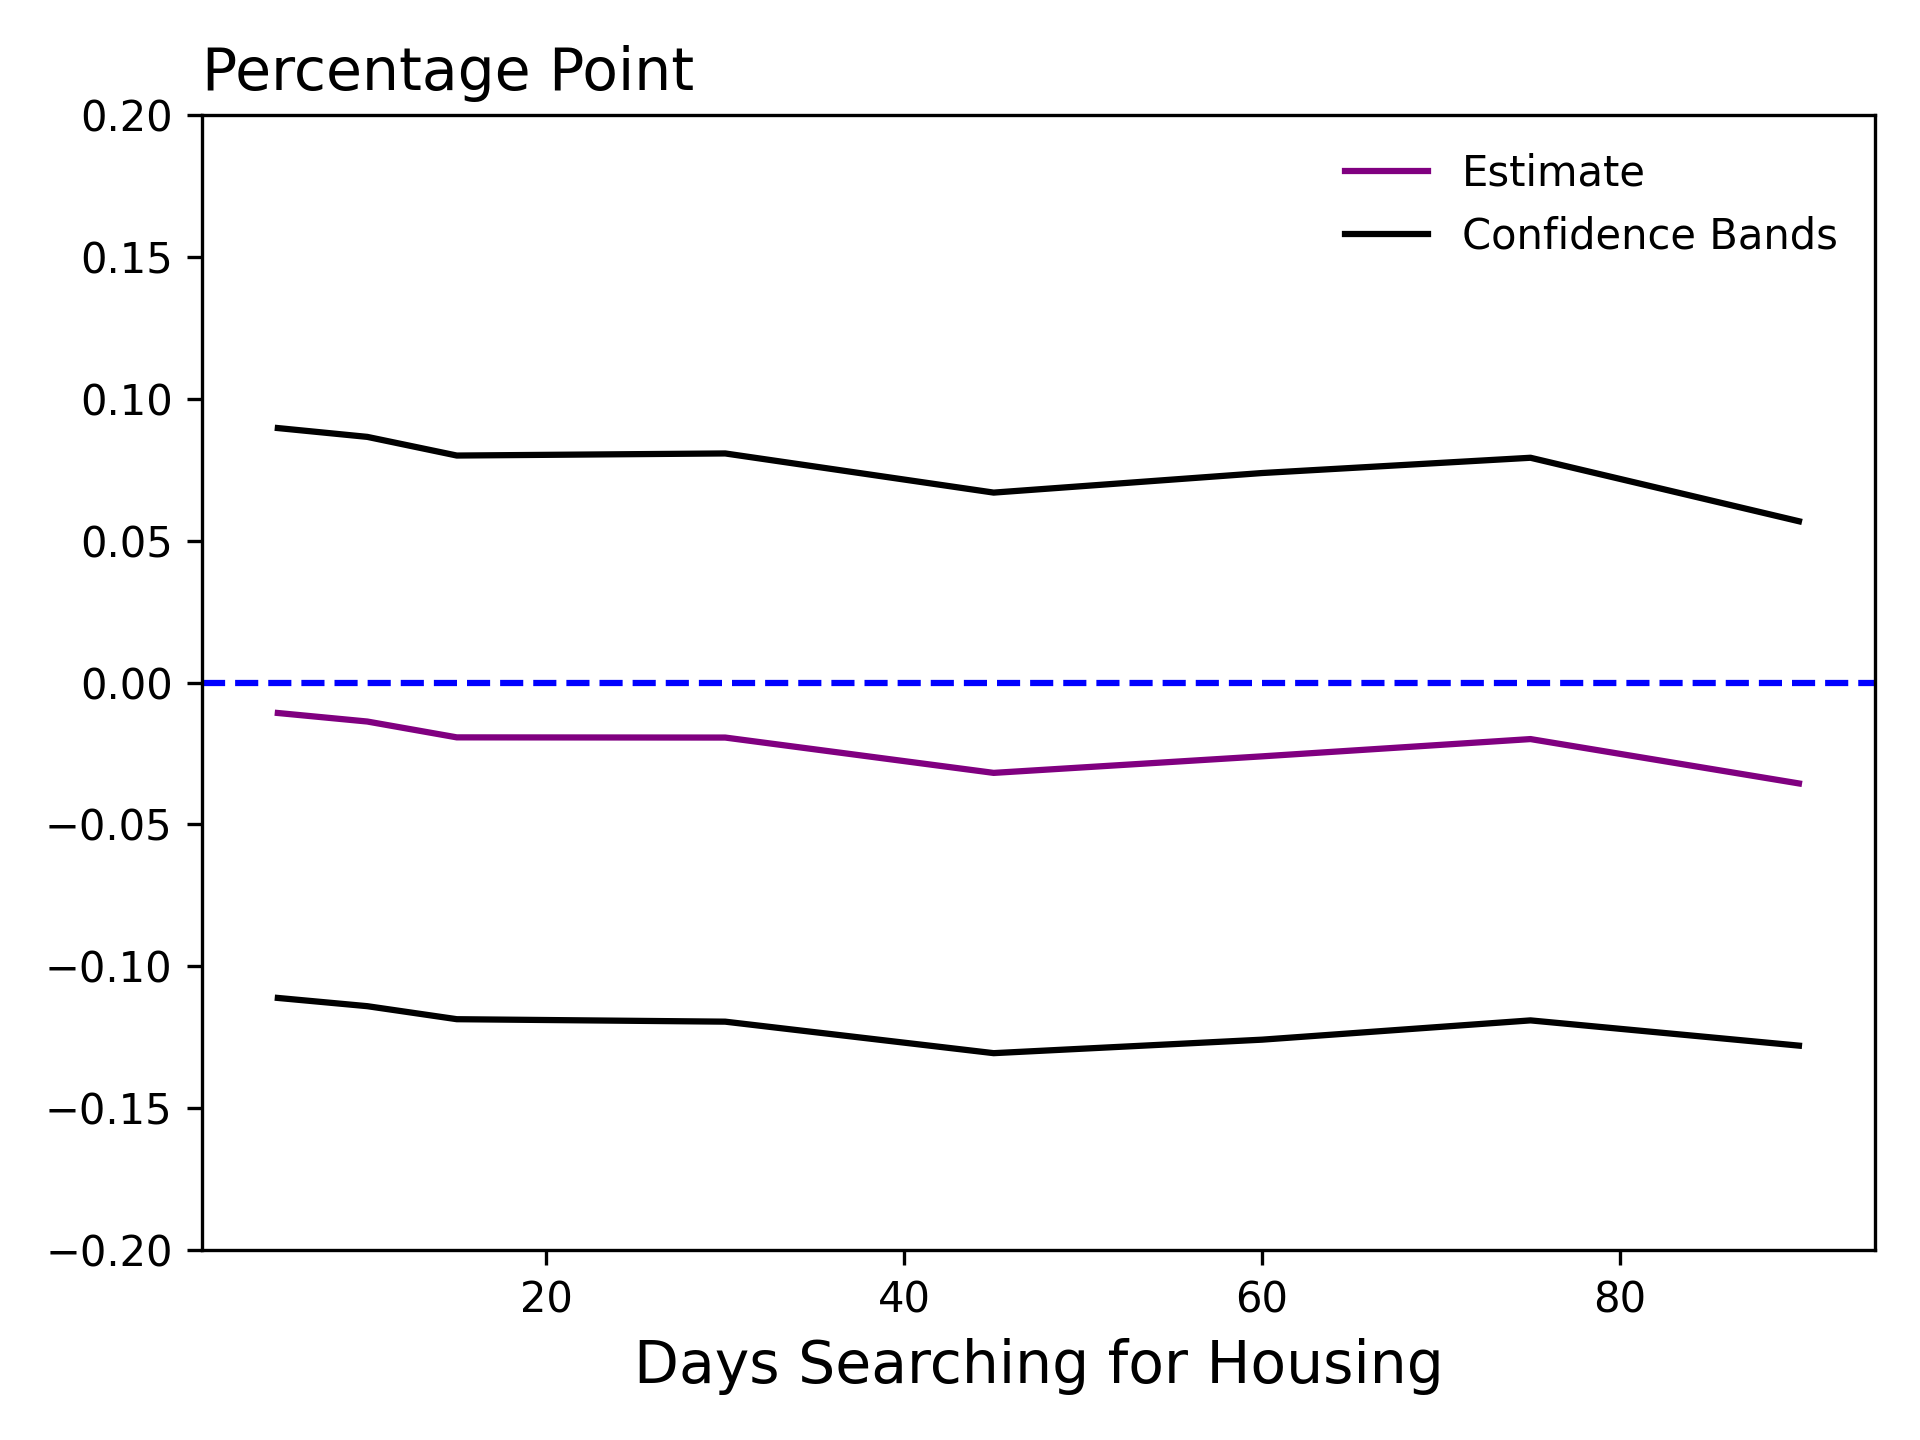
\includegraphics[width=.95\linewidth]{figures/rtc/results/cceh/rfp_False_False.png}
    \caption{All zip codes}
    \label{SUBFIGURE LABEL 3}
\end{subfigure}
\begin{subfigure}{.48\textwidth}
    \centering
    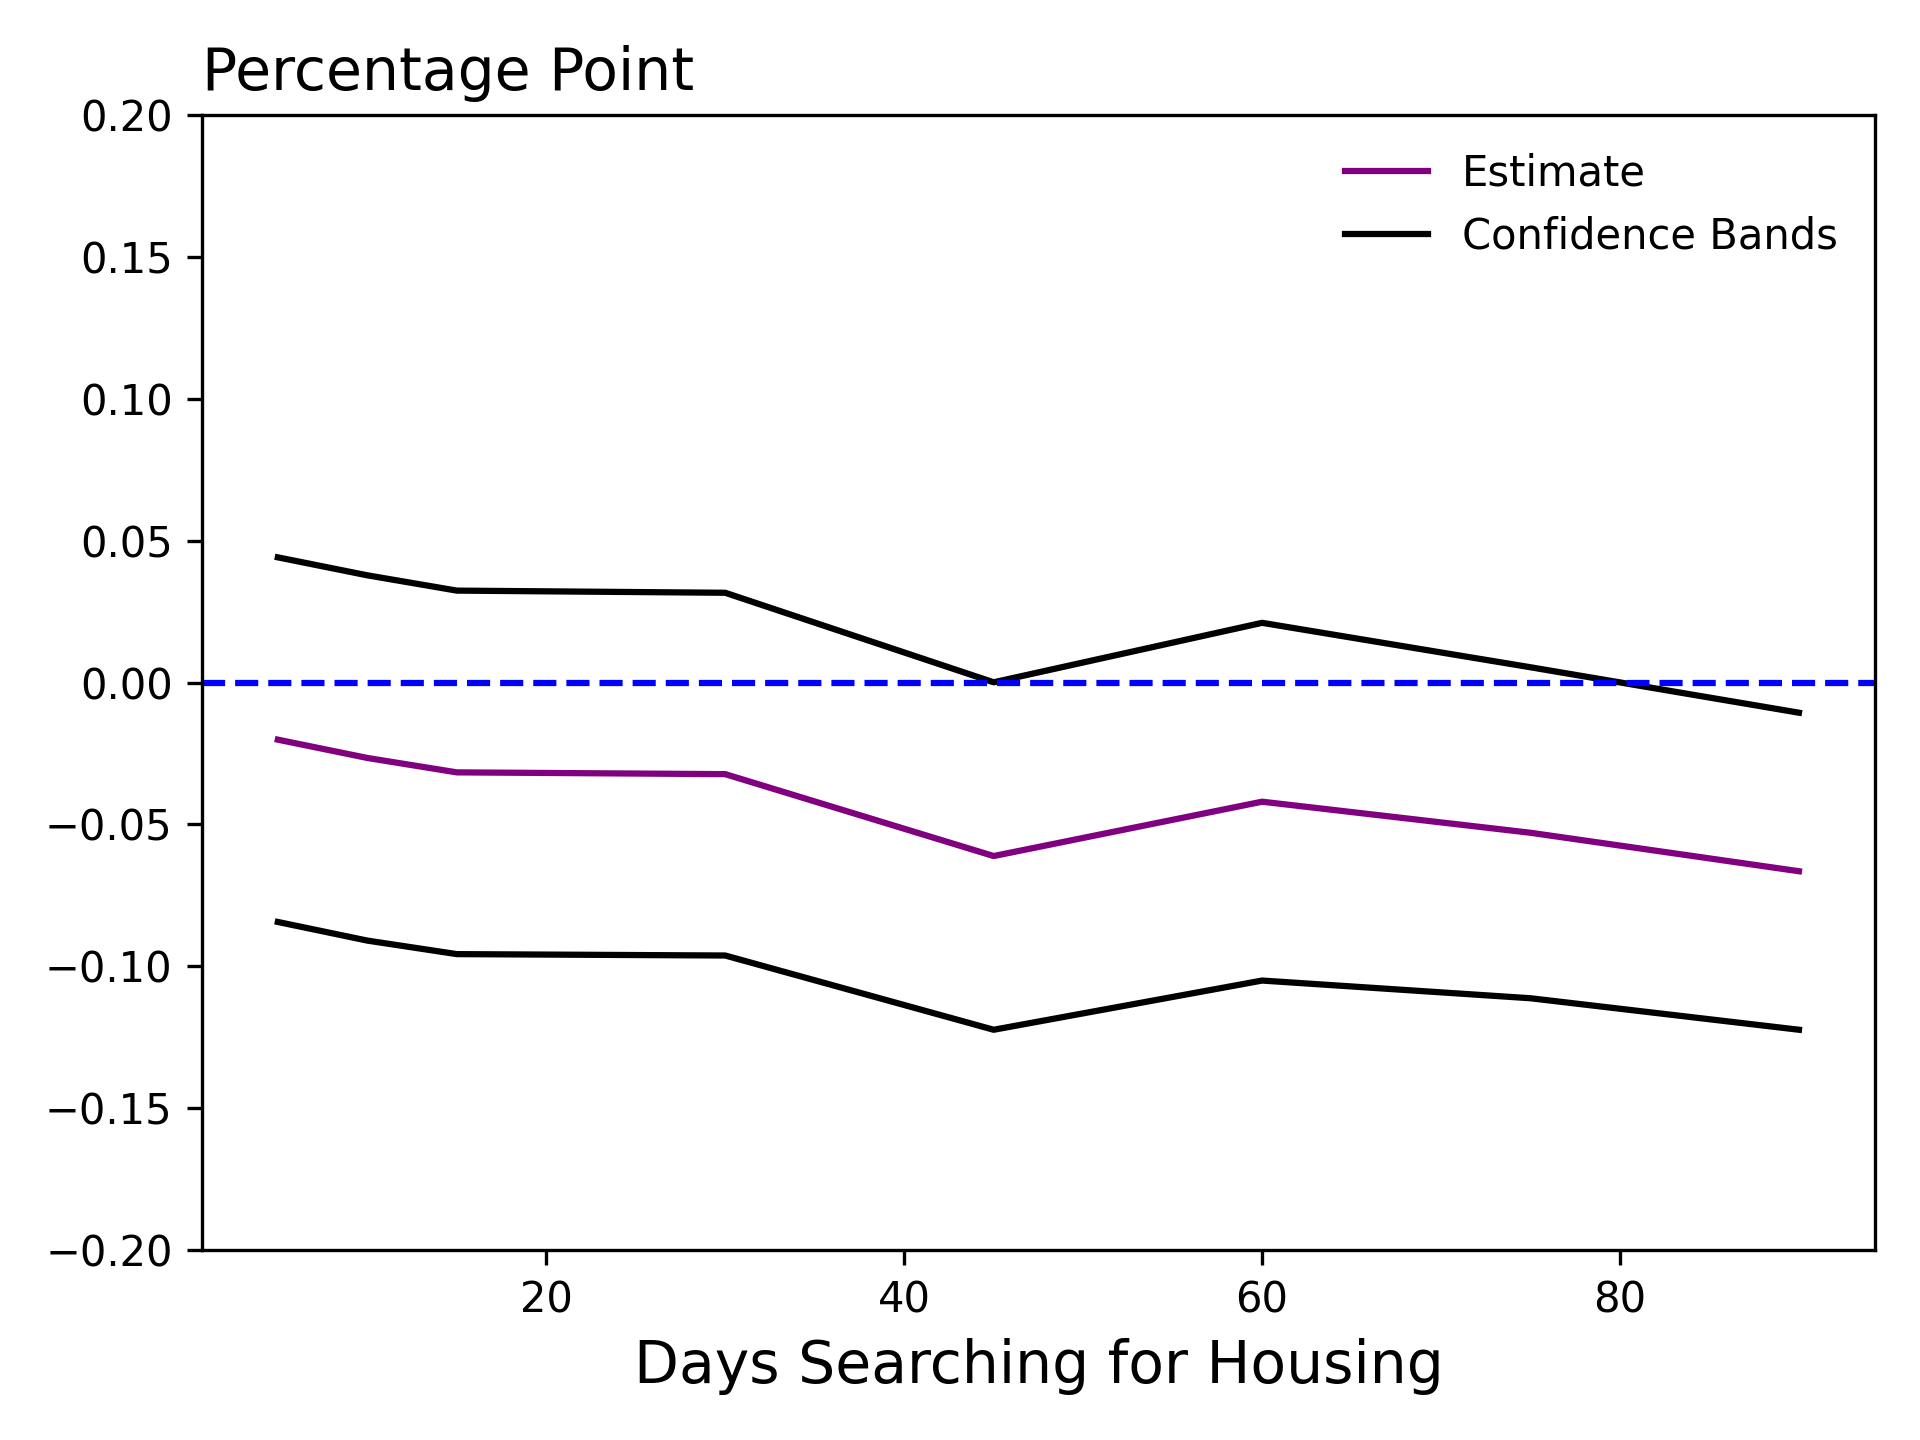
\includegraphics[width=.95\linewidth]{figures/rtc/results/cceh/rfp_True_False.png}
    \caption{High Eviction Zip Codes}
    \label{SUBFIGURE LABEL 4}
\end{subfigure}
\caption{ \href{https://github.com/pharringtonp19/evictions/blob/main/scripts/cceh/primary/cluster_diff_n_diff.py}{Reproduced Here}: Confidence Bands formed sampling across random parameter initializations}
\label{fig:rfp_results}
\end{figure}
While the magnitude of the effect shrinks, the sign of the effect is relatively constant and negative when restricting the sample to high eviction zip codes. We also note that the difference in the estimated effects when considering the all zip codes and only high eviction zip codes decrease. \par 
Over a long time frame, it would be interesting to assess whether the tail of the distribution increased. As \cite{evans2019reducing} notes in summaring previous homelessness related work, the costs are often associated with those in the tail.\footnote{\cite{evans2019reducing} notes that In Spellman et al. (2010), the costliest 10 percent of people incur up to 83 percent of the total costs of shelter
during homelessness. In Flaming et al. (2015), individuals with costs in the top 5 percent of the public costs
incur 47 percent of all costs. Hence, whether a program targets the costliest cases matters significantly for the
mean costs reported above.''}




 
\section{Conclusion}
As a general statement, Economists are interested in understanding the effects of policies at scale. Almost by definition, though, these effects are not well identified. The aim, therefore, is to capture a particular effect of the policy as it's in the process of being deployed with the hope that this intermediate measurement might be informative about the effect under the new equilibrium.\par 
In this paper, we take as our intermediate measurement the housing search length for low-income individuals. As explained in the body of the paper, this is a far from perfect or comprehensive outcomes variable. That said, we regard as a meaningful signal in the sense that if there are adverse effects of the policy -- if landlords decide to re-optimize in an adverse fashion in response to the Right to Counsel -- we would likely see it via the housing search channel. \par 
And indeed, while extremely preliminary, we see some indication that there may be adverse effects along this channel. Across a series of estimators, each of which fits within a general empirical estimation structure of ``Regularizing the Forward Pass'' which we introduce in this paper, we see that search length increases.

%\bibliographystyle{plainnat}
\bibliography{bibliography.bib}

\section{Appendix}
\subsection{Context Plots}
\begin{figure}[htbp]
\centering
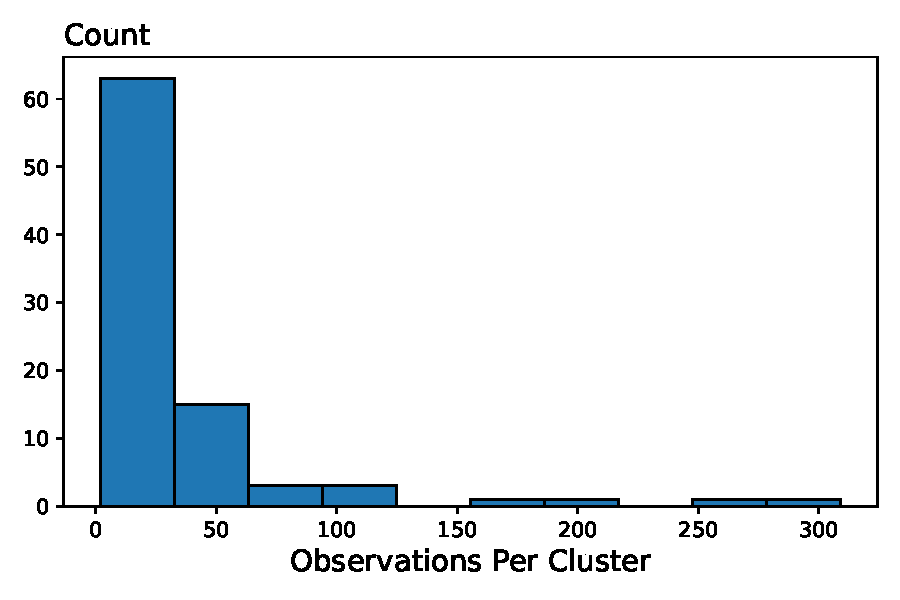
\includegraphics[width=.5\linewidth]{figures/rtc/results/cceh/cluster_dist_False_False.pdf}
\caption{ \href{https://github.com/pharringtonp19/evictions/blob/main/scripts/cceh/primary/diff_n_mean_rrh.py}{Reproduced Here}}
\label{FIGURE LABEL}
\end{figure}
\subsection{High-Level Overview of Model}
\begin{align*}
\intertext{Test}
    &l \circ f \circ c \\ 
\intertext{Training} 
    &l >=> f >=> c \\ 
\end{align*}

\subsection{Category Theory Explanation}
\begin{align*}
&\textrm{class Functor} \ f \ \textrm{where} \\ 
&\quad \textrm{fmap} \ :: \ (a \to b) \to (f \ a \to f \ b) \\ \\ 
&\textrm{instance Functor RFP where} \\ 
&\quad \textrm{fmap} \ f \ (x, r) = (f \ x, g(f) \ x + r)  \\ 
\end{align*}
\begin{quote}
    \textbf{Type Class}: It's not enough to simply restrict the number of iterations of the inner loop. You need to fmap! That is, fmap is regularizing the forward pass: a statistic you compute during the forward pass. To be exact, we're defining a specific functor which is captured in haskell via the implementation of fmap. 
\end{quote}
If we make the simplification that we have two types, Data and Params, then our neural networks models can be thought of as functions between these sets: the clusterMap maps from Params to Params and the featureMap from Params to Data. With this, we have a category. \par 
As explained in section \ref{sec:framework}, during training, we would like our neural network models to return a regularization value in addition to the predictions. We can do so with the help of a functor\footnote{As illustrated via the math, as programmers our functors can be thought of as a type constructor - \cite{milewski2019category}} which maps our category into a new category. For the types, it augments them the the regularization value. And for our neural network models, it embelleshes them so that they return both desired outputs. Just from this, it is then evident that when we are training the model, we are working in one category while during inference we're working in another.\par 
\begin{align*}
\intertext{Type Constructor}
&\textrm{data Reg a} = \textrm{Float} \  \& \ a \\ 
\intertext{fmap}
&\textrm{fmap} :: (a \to b) \to (\textrm{Reg a}  \to \textrm{Reg a} )
\end{align*}
This structure highlights that the key design choice is the fmap (how do you explicitly penalize the neural network).
\subsection{Framework Motivation}
\begin{figure}[htbp]
\centering
\begin{subfigure}{.48\textwidth}
    \centering
    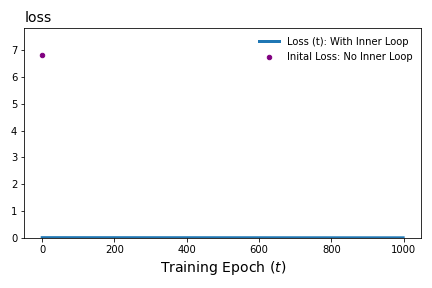
\includegraphics[width=.95\linewidth]{figures/framework/full_inner_loop.png}
    \caption{}
    %\label{SUBFIGURE LABEL 3}
\end{subfigure}
\begin{subfigure}{.48\textwidth}
    \centering
    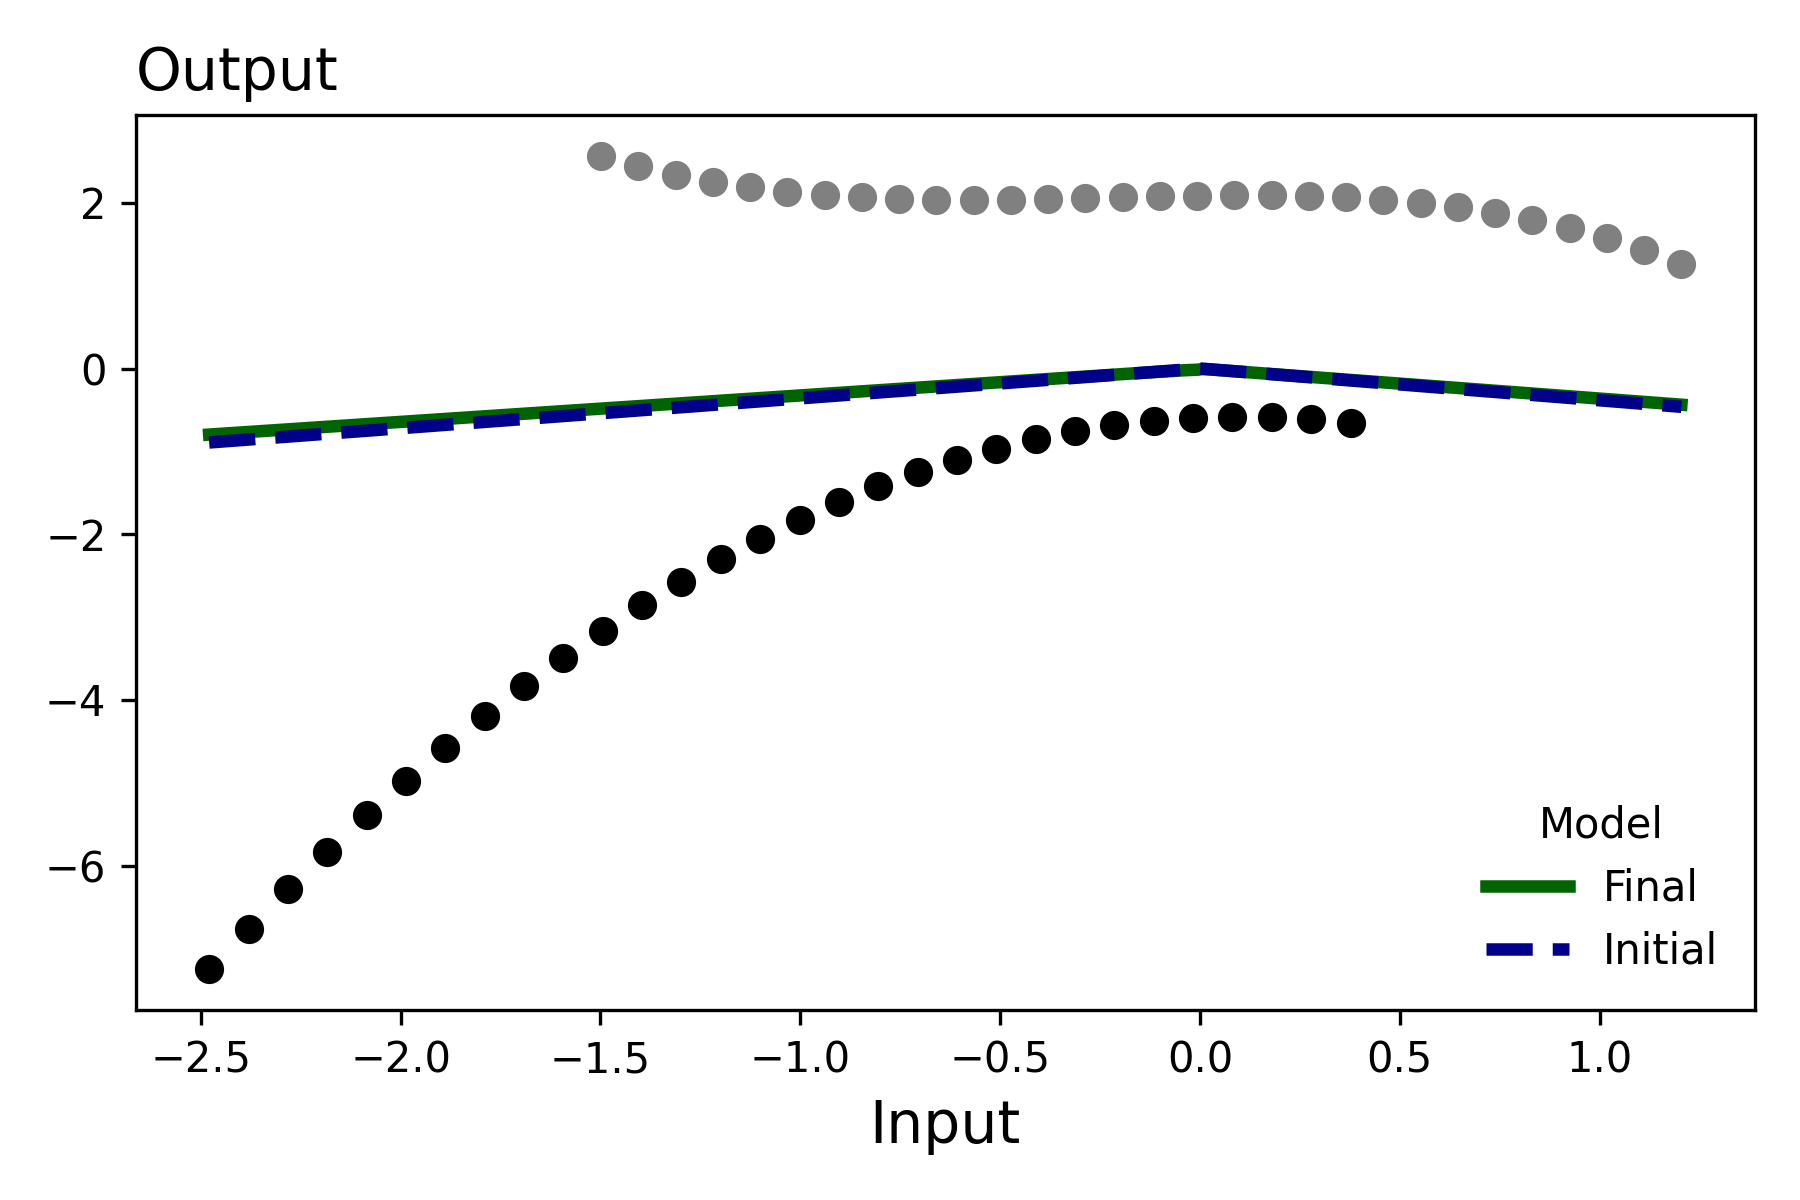
\includegraphics[width=.95\linewidth]{figures/framework/full_inner_loop_models.png}
    \caption{}
    %\label{SUBFIGURE LABEL 4}
\end{subfigure}
\caption{Without regularizing the implicit cluster maps, we risk losing the signal of the gradient -- \href{https://github.com/pharringtonp19/rfp/blob/main/notebooks/Missing_Gradients.ipynb}{Reproduced Here}}
\label{fig:Missinggrads}
\end{figure}
\subsection{Loss Function}
\begin{align*}
    \hat{\theta} &= \underset{\theta}{\textrm{argmin}}\ \mathcal{L}(\theta) \\ 
    &= \underset{\theta}{\textrm{argmin}}\ \sum _c \mathcal{L}_c(\theta)\\ 
    &= \underset{\theta}{\textrm{argmin}}\ \sum _c  F(\theta, \theta^*_c(\theta))\\
    &= \underset{\theta}{\textrm{argmin}}\ \sum _c  F(\theta, \underset{\theta_c}{\textrm{argmin}} \ F(\theta, \theta_c) )\\
\end{align*}
\subsection{Haskell-like Signatures}
\begin{align*} 
&\text{regMAML} :: \text{Data} \rightarrow \text{Params} \rightarrow \big(\textrm{Params}, \text{Float}\big) \\
&\text{regMAML} \ \textcolor{blue}{\text{data}} \ \textcolor{purple}{\theta} := \Big(\text{Update}_m \circ \text{Update}_{m-1} \dots \circ \text{Update}_1 \Big) \ \textcolor{purple}{\theta}, \quad \mathcal{L}_c(\textcolor{blue}{\text{data}}, \textcolor{purple}{\theta})  \\ 
&  \quad \quad \quad \quad \quad \quad \quad \quad \quad \quad \text{where} \quad  \text{Update}_t \  \theta = \theta - \alpha_t \nabla \mathcal{L}_c(\textcolor{blue}{\text{data}}, \textcolor{purple}{\theta})
\end{align*}
\begin{align*}
    &\text{regNeuralODE} :: \text{Data} \rightarrow \text{Params} \rightarrow \big(\textrm{Data}, \text{Float}\big) \\
&\text{regNeuralODE} \ \_ \ \textcolor{blue}{x} \ \_ \ \textcolor{purple}{\theta} := x + \int f(t, x(t), \theta)dt, \quad \int \Big\| \frac{\partial ^k}{dt^k}f(t, x(t), \theta) \Big\|dt \\ 
& \quad \quad \quad \quad \quad \quad \quad \quad \quad \quad \text{where}  \quad x(0)=x \\ \\ 
\end{align*}
\subsection{Method Implementation}
\begin{figure}[htbp]
\centering
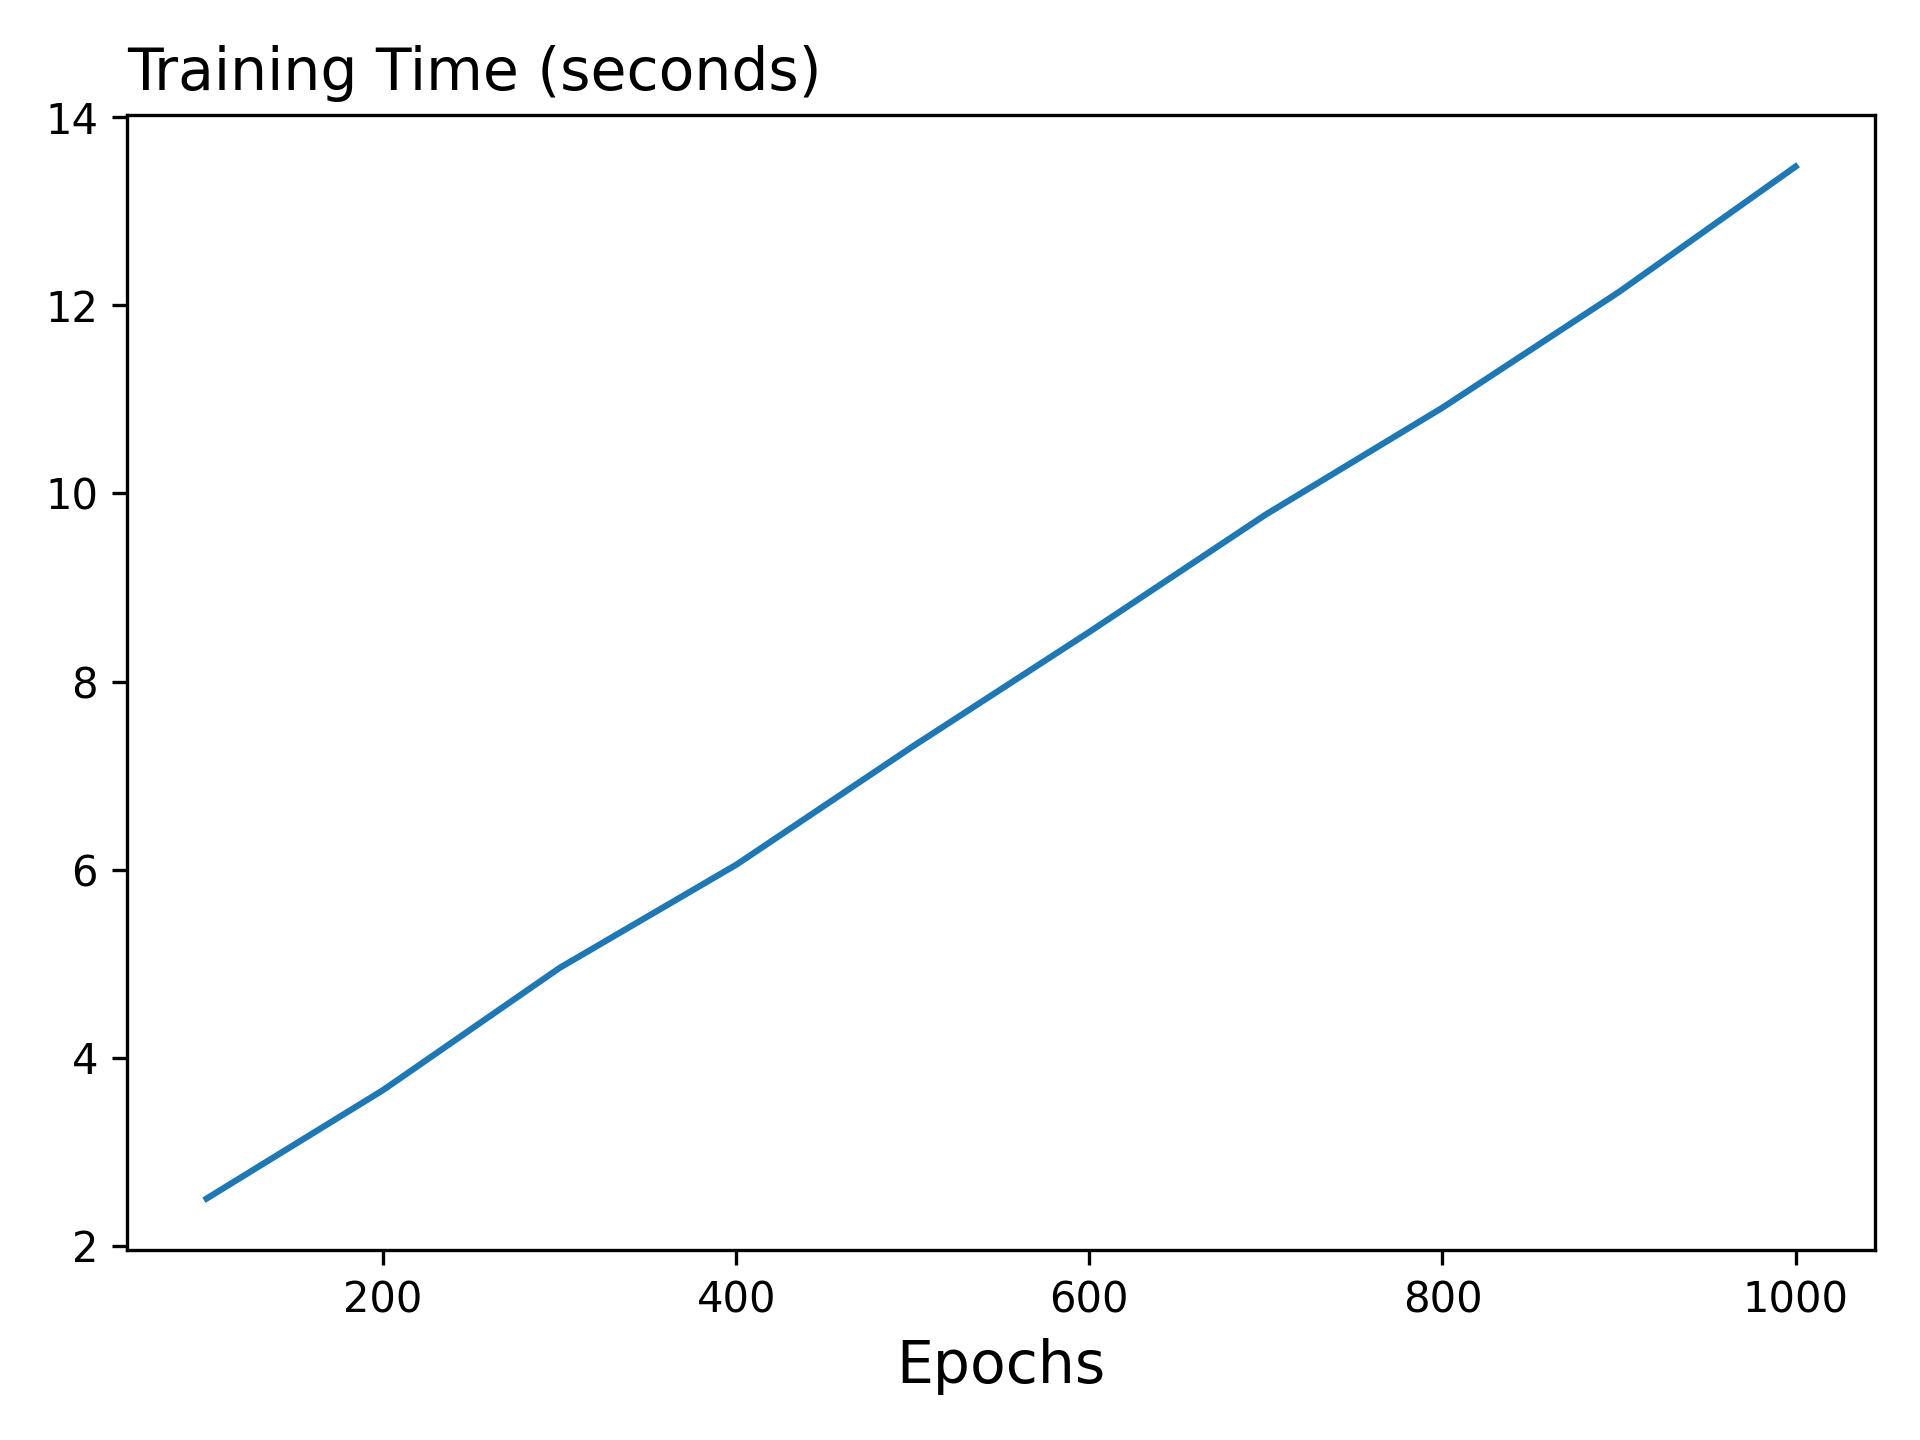
\includegraphics[width=.5\linewidth]{figures/framework/method_time.png}
\caption{ \href{https://github.com/pharringtonp19/evictions/blob/main/scripts/method/time_train_plot.py}{Reproduced Here}}
\label{FIGURE LABEL}
\end{figure}

\begin{figure}[htbp]
\centering
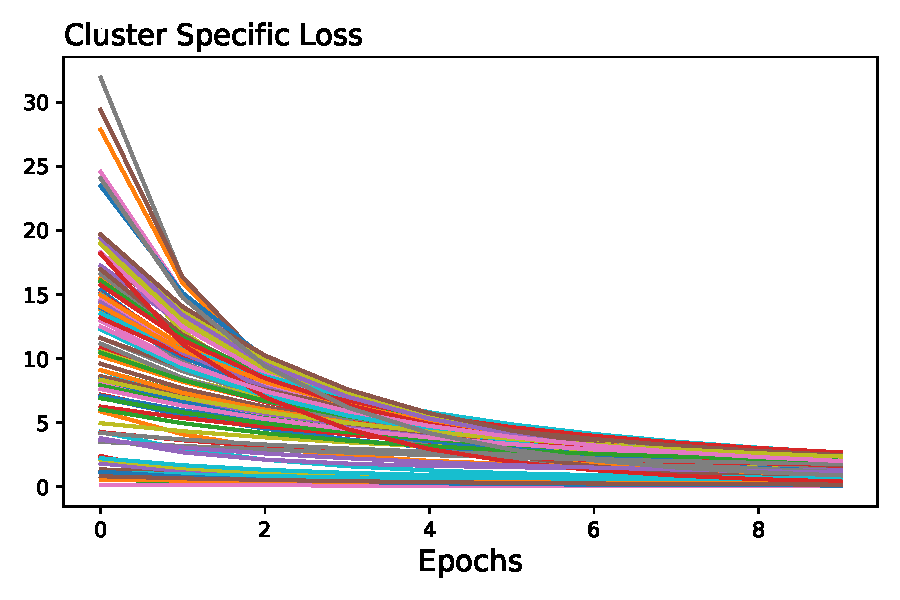
\includegraphics[width=.5\linewidth]{figures/framework/inner_loop_0.pdf}
\caption{ \href{https://github.com/pharringtonp19/evictions/blob/main/scripts/cceh/primary/diff_n_mean_rrh.py}{Reproduced Here}}
\label{FIGURE LABEL}
\end{figure}

\end{document} 

